\documentclass[12pt,openany]{book}
\usepackage[utf8]{inputenc}
\usepackage[T1]{fontenc}
\usepackage[dvips,a4paper,hmargin={2cm,2cm},vmargin={2cm,2cm}]{geometry}
\usepackage[a4paper,colorlinks=true,bookmarksopen=false,linkcolor=brown,citecolor=red]{hyperref}
\usepackage{pythontex}
\usepackage{calc}
\usepackage{comment}
\usepackage{amssymb}
\usepackage{amsthm}
\usepackage{amsmath}
\usepackage{amsrefs}
\usepackage{titlesec}
\usepackage{titletoc}
\usepackage{dsfont}
\usepackage{euscript}
\usepackage{fourier-orns}
\usepackage{fontawesome}
\usepackage{palatino}
\usepackage{graphicx}
\usepackage{tikz-cd}
\tikzcdset{
arrow style=tikz,
diagrams={>=latex}
}

\def\RR{\mathds R}
\def\ZZ{\mathds Z}
\def\NN{\mathds N}
\def\QQ{\mathds Q}
\def\P{\EuScript P}
\def\0{\varnothing}
\def\E{{\rm E}}
\def\Var{{\rm Var}}
\def\range{\mathop{\rm img}}
\linespread{1.2}
\setlength{\parindent}{0ex}
\setlength{\parskip}{.5\baselineskip}

% \DeclareFontFamily{OT1}{pzc}{}
% \DeclareFontShape{OT1}{pzc}{m}{it}{<-> s * [1.10] pzcmi7t}{}
% \DeclareMathAlphabet{\mathpzc}{OT1}{pzc}{m}{it} 


\newcommand{\mylabel}[1]{{\footnotesize\textsf{#1}}\hfill}
\renewenvironment{itemize}
  {\begin{list}{$\triangleright$}{%
   \setlength{\parskip}{0mm}
   \setlength{\topsep}{.2\baselineskip}
   \setlength{\rightmargin}{0mm}
   \setlength{\listparindent}{0mm}
   \setlength{\itemindent}{0mm}
   \setlength{\labelwidth}{3ex}
   \setlength{\itemsep}{.4\baselineskip}
   \setlength{\parsep}{0mm}
   \setlength{\partopsep}{0mm}
   \setlength{\labelsep}{1ex}
   \setlength{\leftmargin}{\labelwidth+\labelsep}
   \let\makelabel\mylabel}}{%
   \end{list}\vspace*{-1.3mm}}

   
\definecolor{blue}{rgb}{0, 0.1, 0.6}
\def\emph#1{\textcolor{blue}{\textbf{\boldmath #1}}}

\def\theta{\vartheta}
\def\phi{\varphi}
\def\epsilon{\varepsilon}
\def\ssf#1{\textsf{\small #1}}

\titlecontents{section}
[3.8em] % ie, 1.5em (chapter) + 2.3em
{\vskip-1ex}
{\contentslabel{1.5em}}
{\hspace*{-2.3em}}
{\titlerule*[1pc]{}\contentspage}


\titleformat
{\chapter} % command
[display] % shape
{\bfseries\LARGE} % format
{Chapter \ \thechapter} % label
{0.5ex} % sep
{} % before-code
[] % after-code
\titleformat{\section}[block]{\Large\bfseries}{\makebox[5ex][r]{\textbf{\thesection}}}{1.5ex}{}
\titlespacing{\subsection}{0ex}{.5ex plus .5ex minus .5ex}{1ex plus .2ex minus .2ex}
\titlespacing*{\chapter}{0em}{.5ex plus .2ex minus .2ex}{2.3ex plus .2ex}
\titlespacing*{\section}{-9.7ex}{3ex plus .5ex minus .5ex}{1ex plus .2ex minus .2ex}

\renewcommand*\thesection{\arabic{section}}

\newtheoremstyle{mio}% name
     {2\parskip}%      Space above
     {\parskip}%      Space below
     {\sl}%         Body font
     {}%         Indent amount (empty = no indent, \parindent = para indent)
     {\bfseries}% Thm head font
     {}%        Punctuation after thm head
     {1.5ex}%     Space after thm head: " " = normal interword space;
           %   \newline = linebreak
     {\llap{\thmnumber{#2}\hskip2mm}\thmname{#1}\thmnote{\bfseries{} #3}}% Thm head spec (can be left empty, meaning `normal')

\newtheoremstyle{liscio}% name
     {2\parskip}%      Space above
     {0mm}%      Space below
     {}%         Body font
     {}%         Indent amount (empty = no indent, \parindent = para indent)
     {\bfseries}% Thm head font
     {}%        Punctuation after thm head
     {1.5ex}%     Space after thm head: " " = normal interword space;
           %   \newline = linebreak
     {\llap{\thmnumber{#2}\hskip2mm}\thmname{#1}\thmnote{\bfseries{} #3}}% Thm head spec (can be left empty, meaning `normal')

\newcounter{thm}[chapter]

\renewcommand{\thethm}{\thechapter.\arabic{thm}}

\theoremstyle{mio}
\newtheorem{theorem}[thm]{Theorem}
\newtheorem{corollary}[thm]{Corollary}
\newtheorem{proposition}[thm]{Proposition}
\newtheorem{lemma}[thm]{Lemma}
\newtheorem{fact}[thm]{Fact}
\newtheorem{void_thm}[thm]{}
\newtheorem{definition}[thm]{Definition}
\theoremstyle{liscio}
\newtheorem{void_def}[thm]{}
\newtheorem{remark}[thm]{Remark}
\newtheorem{notation}[thm]{Notation}
\newtheorem{note}[thm]{Note}
\newtheorem{exercise}[thm]{Exercise}
\newtheorem{example}[thm]{Example}
\setlength{\partopsep}{0mm}
\setlength{\topsep}{0mm}
\def\QED{\noindent\nolinebreak[4]\hfill\rlap{\ \ $\Box$}\medskip}
\renewenvironment{proof}[1][Proof]%
{\begin{trivlist}\item[\hskip\labelsep {\bf #1}]}
{\QED\end{trivlist}}

\newenvironment{void}[1][]%
{\begin{trivlist}\item[\hskip\labelsep {\bf #1}]}
{\QED\end{trivlist}}



\pagestyle{empty}

\definecolor{violet}{RGB}{115, 0, 205}
\definecolor{brown}{RGB}{150, 50, 10}
\definecolor{green}{RGB}{10,120, 20}
\def\mr{\color{brown}}
\def\gr{\color{green}}
\def\vl{\color{violet}}



\begin{document}
\setlength{\abovedisplayskip}{-1ex}
\setlength{\belowdisplayskip}{0pt}




\chapter{Teoria (il minimo sindacale)}
\raggedbottom

Per esempi e esercizi seguire i \hyperref[ch2]{link \faShare}

%%%%%%%%%%%%
%%%%%%%%%%%%
%%%%%%%%%%%%
\clearpage\section{Spazio di probabilità}

{\color{brown}Esempi: \hyperref[tetraedro]{Dado a $4$ facce \faShare}
\\
\hphantom{Esempi:} \hyperref[doppo_lancio_moneta]{Doppio lancio moneta \faShare}
\\
\hphantom{Esempi:} \hyperref[urna_3_colori]{Urna con biglie di 3 colori \faShare}}





\def\medrel#1{\parbox[t]{6ex}{$\displaystyle\hfil #1$}}
\def\ceq#1#2#3{\parbox{25ex}{$\displaystyle #1$}\medrel{#2}$\displaystyle  #3$}


Fisssiamo un insieme non vuoto \emph{$\Omega$\/} che chiameremo \emph{spazio campionario\/}  (\emph{sample space\/}) o \emph{popolazione}. Immagimiamo gli elementi \emph{$\omega$\ }$\in\Omega$ come i possibili \emph{risultati\/} di un rilevamento, un esperimento, un sorteggio, ecc. I sottoinsiemi $E\subseteq\Omega$ verranno chiamati \emph{eventi\/} e, intuitivamente, rapresentano proprietà osservabili.

Una \emph{misura di probabilità\/} è una funzione $\Pr:\P(\Omega)\to\RR$ tale che 

\begin{itemize}
\item $\Pr(\Omega)=1$
\item $\Pr(E)\ge0$ per ogni $E\in\P(\Omega)$
\item $\Pr(E_1\cup E_2)=\Pr(E_1)+\Pr(E_2)$ per ogni coppia $E_1,E_2\in\P(\Omega)$ di insiemi \emph{disgiunti}, ovvero $E_1\cap E_2=\0$. Si dice anche che $E_1$ e $E_2$ sono \emph{eventi mutualmente esclusivi}.
\end{itemize}

Conseguenze:


\begin{itemize}
\item $\Pr(\0)=0$
\item $\Pr(\neg E)=1-\Pr(E)$
%\item $\Pr(E_1\cup E_2\cup E_3)=\Pr(E_1)+\Pr(E_2)+\Pr(E_3)$ per ogni $E_1,E_2,E_3$ mutualmente esclusivi.
\item $\Pr(E_1\smallsetminus E_2)=\Pr(E_1)-\Pr(E_2)$ se $E_2\subseteq E_1$
\item $\Pr(E_1\cup E_2)=\Pr(E_1)+\Pr(E_2)-\Pr(E_1\cap\E_2)$ per ogni coppia $E_1,E_2\in\P(\Omega)$.
\end{itemize}

%%%%%%%%%%%%
%%%%%%%%%%%%
%%%%%%%%%%%%
\clearpage\section{Variabili aleatorie}


\def\medrel#1{\parbox[t]{6ex}{$\displaystyle\hfil #1$}}
\def\ceq#1#2#3{\parbox{25ex}{$\displaystyle #1$}\medrel{#2}$\displaystyle  #3$}


Sia $R$ un insieme quasiasi. Una \emph{variabile aleatoria\/} è una funzione $X:\Omega\to R$. Se $R$ è un insieme numerico (un sottoinsieme di $\NN$, $\ZZ$, $\QQ$, $\RR$, $\RR^2$, ecc.) diremo che $X$ è una \emph{variabile aleatoria numerica}. Una variabile aleatoria non numerica è detta \emph{qualitativa\/} o \emph{categorica}.


%%%%%%%%%%%%
%%%%%%%%%%%%
%%%%%%%%%%%%
\clearpage\section{Distribuzione di probabilità discreta}

Come sopra $X:\Omega\to R$ è una variabile aleatoria. Dato $x\in R$ e $A\subseteq R$ scriveremo

\ceq{\hfill \emph{$p_x$}\medrel{=}\emph{$\Pr(X=x)$}}{=}{\Pr\big(\{\omega\in\Omega\ :\ X(\omega)=x)\}\big)}

\ceq{\hfill \emph{$\Pr(X\in A)$}}{=}{\Pr\big(\{\omega\in\Omega\ :\ X(\omega)\in A)\}\big)}

\ceq{\hfill \emph{$\Pr(X \le x$)}}{=}{\Pr\big(\{\omega\in\Omega\ :\ X(\omega)\le x)\}\big)}\hfill  se $X$ \`e numerica.

La funzione $\Pr(X=x)$ si chiama \emph{distribuzione di probabilità (probability mass function)}. La funzione $\Pr(X \le x)$ si chiama  \emph{funzione di ripartizione (cumulative distribution function)}.

Le variabili numeriche possono dirsi \emph{discrete\/} o \emph{continue}. Una v.a.\@ $X$ è discreta se per ogni sottoinsieme $A\subseteq R$

\ceq{\hfill \Pr\big(X\in A\big)}{=}{\sum_{x\in A}\Pr(X=x)}

Ovvero la probabilità è concentrata nei punti di $R$. Invece una variabile continua se $\Pr(X{=}x)=0$ per ogni $x\in R$. Per le variabili continue è significativa solo la probabilità in intervalli di diametro positivo


\ceq{\hfill \Pr\big(X\in [a,b]\big)}{=}{\Pr(a \le X \le b)\medrel{=}\Pr(X\le b)-\Pr(X\le a)}

Si noti che la seconda uguaglianza non sarebbe corretta se $\Pr(X{=}a)\neq0$.

N.B. Esistono variabili aleatorie (anche in esempi concreti) che sono intermedie tra il continuo e il discreto ma per il momento non le considereremo.



%%%%%%%%%%%%
%%%%%%%%%%%%
%%%%%%%%%%%%
\clearpage\section{Variabili aleatorie di Bernoulli}

Una variabile aleatoria $X$ si dice di bernulli se \emph{Bernoulli\/} se $\range X=\{0,1\}$.

Possiamo identificare in modo canonico eventi e variabili aletorie di Bernoulli. L'evento associato ad $X$ è l'insieme $\{\omega:X(\omega)=1\}$ che chiameremo \emph{successo}. Chiameremo \emph{$p$}\ $ = \Pr(X{=}1)$ la \emph{probabilità di successo}.

Viceversa, la v.a.\@ di Bernoulli associata ad un evento $E$ è spesso denotata con $1_E$

\ceq{\hfill 1_E(x)}{=}{\left\{\begin{array}{ll}1&\textrm{ se }\ x\in E\\0&\textrm{ se }\ x\notin E\end{array}\right.}

Per dire che $X$ è una variabile aleatoria di Bernoulli con probabilità di successo $p$ scriveremo \emph{$X\sim B(1,p)$}.



%%%%%%%%%%%%
%%%%%%%%%%%%
%%%%%%%%%%%%
%%%%%%%%%%%%
\clearpage\section{Probabilità condizionata} 

{\color{brown}Esempi: \hyperref[MF_totali]{Popolazione maschile e femminile (probabilità totali) \faShare}
\\
\hphantom{Esempi:} \hyperref[Fumatori_Bayes]{Fumatori (regola di Bayes) \faShare}
\\
\hphantom{Esempi:} \hyperref[rain_desert]{Rain forcasts (Bayes rule) \faShare}}


Dato $A, \Phi\subseteq\Omega$ tali che $\Pr(\Phi)\neq 0$ definiamo 

\ceq{\hfill \emph{$\Pr(A\mathbin|\Phi)$}}{=}$\displaystyle\frac{\Pr(A\cap\Phi)}{\Pr(\Phi)\vphantom{\Big[}}$

Questo si legge \emph{probabilità di $A$ dato $\Phi$}. Si verifica facilmente che $\Pr(\,\cdot\,|\Phi)$ soddisfa a tutte le propriet\`a di $\Pr(\,\cdot\,$) se rimpiazziamo $\Omega$ con $\Phi$.

Il fatto seguente si chiama \emph{Teorema delle Probabilità Totali}: siano $A_1,\dots,A_n$ eventi \emph{mutuamente esclusivi\/} ed \emph{esaustivi} di probabilità $\neq0$. Sia $C$ \`e un qualsiasi altro evento, allora

\ceq{\hfill \Pr(C)}{=}{\sum^n_{i=1} \Pr(A_i)\cdot \Pr\big(C| A_i).}

Il seguente di chiama \emph{Teorema (o regola) di Bayes}: per ogni coppia di eventi $A$ e $B$ di probabilit\`a $\neq0$ 

\ceq{\hfill \Pr(A|B)}{=}{\frac{\Pr(B|A)\cdot \Pr(A)}{\Pr(B)\vphantom{\Big[}}.}

In molte applicazioni $\Pr(B)$ viene calcolato usanto il teorema delle probabilità totali.

\ceq{}{=}{\frac{\Pr(B|A)\cdot \Pr(A)}{\Pr(B|A)\Pr(A)+\Pr(B|\neg A)\Pr(\neg A)\vphantom{\Big[}}.}


%%%%%%%%%%%%%%%%%%%%%%%
%%%%%%%%%%%%%%%%%%%%%%%
%%%%%%%%%%%%%%%%%%%%%%%
%%%%%%%%%%%%%%%%%%%%%%%
\clearpage\section{Indipensenza stocastica}

Due eventi $A$ e $B$ si dicono \emph{(stocasticamente) indipenenti\/} se 

\ceq{\hfill \Pr(A\cap B)}{=}{\Pr(A)\cdot \Pr(B)}. 

Il seguente fatto è facile da verificare: se $A$ e $B$ sono eventi probabilità non nulla allora sono indipendenti se e solo se $\Pr(A|B)=\Pr(A)$ se e solo se $\Pr(B|A)=\Pr(B)$.

Due variabili aleatorie discrete $X$ ed $Y$ si dicono \emph{(stocasticamente) indipenenti\/} se per ogni $x\in\range X$ e $y\in\range Y$

\ceq{\hfill \Pr(X, Y =x,y)}{=}{\Pr(X=x)\cdot \Pr(Y=y)}.

Nel caso di variabili aleatorie continue la condizione diventa


\ceq{\hfill \Pr(X\le x\ \textrm{ and }\ Y\le y)}{=}{\Pr(X\le x)\cdot \Pr(Y\le y)}.



%%%%%%%%%%%%%%%%%%%%%%%
%%%%%%%%%%%%%%%%%%%%%%%
%%%%%%%%%%%%%%%%%%%%%%%
%%%%%%%%%%%%%%%%%%%%%%%
\clearpage\section{Esperimenti ripetuti: prodotto di spazi di probabilità}

Sia $X:\Omega\to\{0,1\}$ una variabile aleatoria di Bernoulli (per avere un esempio semplice). Immaginiamo che $X$ modelli il lancio di una moneta. Per brevità definiamo $A=X^{-1}[\,1\,]$.

Il lancio ripetuto di una monetina è modellato con lo spazio campionario $\Omega^2$. L'insieme  $A\times\Omega$ è l'evento dello spazio $\Omega^2$ che corrisponde  ad ottenere $1$ nel primo lancio. L'insieme $\Omega\times\!\neg A$ corrisponde ad ottenere $0$ nel secondo lancio.

L'intersezione di questi eventi è $A\times\!\neg A$. Questo corrisponde ad ottenere nei due lanci la sequenza $1\,0$. 

La probabilità di un evento $A\times B\subseteq\Omega^2$ è per definizione $\Pr(A)\cdot \Pr(B)$. Gli eventi $A\times\Omega$ e $\Omega\times B$ sono quindi indipendenti.




%%%%%%%%%%%%%%%%%%%%%%%
%%%%%%%%%%%%%%%%%%%%%%%
%%%%%%%%%%%%%%%%%%%%%%%
%%%%%%%%%%%%%%%%%%%%%%%
\clearpage\section{Variabili aleatorie binomiali}






%%%%%%%%%%%%%%%%%%%%%%%
%%%%%%%%%%%%%%%%%%%%%%%
%%%%%%%%%%%%%%%%%%%%%%%
%%%%%%%%%%%%%%%%%%%%%%%
\clearpage\section{Valore atteso e varianza}

Il \emph{valore atteso\/} o \emph{media di popolazione\/} (\emph{expected value, population mean\/}) di una variabile aleatoria numerica discreta $X$ a valori in $R$ è

\ceq{\hfill\emph{$\mu\medrel{=} \E(X)$}}{=}{\sum_{x\in R} x\cdot \Pr(X=x)}

La \emph{varianza\/} di una variabile aleatoria numerica discreta $X$ a valori in $R$ è

\ceq{\hfill\emph{$\sigma^2\medrel{=} \Var(X)$}}{=}{\sum_{x\in R} \big(x- E(X)\big)^2\cdot \Pr(X=x)}

\ceq{}{=}{E(X^2)-E(X)^2}\hfill (facile da verificare).

La \emph{deviazione standard\/} è la radice della varianza

\ceq{\hfill \emph{$\sigma$}}{=}{\sqrt{\Var(X)\vphantom{\big[]}}}

Le lettere $\mu$ e $\sigma$ vengono usate quando è chiaro a quale variabile ci si riferisce. per evitare ambiguità a volte si scrive $\mu_X$ e $\sigma_X$.




%%%%%%%%%%%%%%%%%%%%%%%
%%%%%%%%%%%%%%%%%%%%%%%
%%%%%%%%%%%%%%%%%%%%%%%
%%%%%%%%%%%%%%%%%%%%%%%
\clearpage\section{Standardizzazione}

Sia $X$ una v.a.\@ con media $\mu$ e deviazione standaed $\sigma$. La variabile aleatoria $Z$ così definita

\ceq{\hfill Z}{=}{\frac{X-\mu}{\sigma}}

si dice ottenuta da $X$ per \emph{standardizzazione}. La variabile $Z$ ha media nulla e deviazione standaed $1$ ed è sempre adimensionale. Un valore ottenuto da $Z$ si dice \emph{punteggio $Z$\/} o \emph{punteggio standard\/} (\emph{$Z$-score}).





%%%%%%%%%%%%
%%%%%%%%%%%%
%%%%%%%%%%%%
\clearpage\section{Diagnostic tests}


{\color{brown}Esempi:}  \hyperref[HIV_test]{HIV test (regola di Bayes) \faShare}
% \\
% \hphantom{Esempi:}

Let \emph{$T_+$\/} and \emph{$T_-$\/} be the events that the result of a diagnostic test
is positive or negative respectively. Let \emph{$D$\/} be the event that the subject of the test has the disease. 

Introduciamo un po di terminologia.

\begin{itemize}
\item We call $\Pr(D)$ the \emph{prevalence\/} of the disease. Often it is very difficult to estimate: it strongly depends on the risk category the subject belongs to.
\item The \emph{sensitivity\/} is the probability that the test is
positive given that the subject actually has the disease, $\Pr(T_+ | D)$
\item The \emph{specificity\/} is the probability that the test is
negative given that the subject does not have the disease, $\Pr(T_- | \neg D)$
\item The \emph{positive predictive value\/} is the probability that the subject has the
disease given that the test is positive, $\Pr(D | T_+)$
\item The \emph{negative predictive value\/} is the probability that the subject does not have
the disease given that the test is negative, $\Pr(\neg D | T_-)$
\item The \emph{prevalence of the disease\/} is the marginal probability of disease, $\Pr(D)$

\end{itemize}


Tipicamente la specificità e la sensitività del test sono note. I poteri predittivi positivi e negativi vengono calcolati usando la prevalenza e regola di Bayes e quindi dipendono fortemente dalla categoria di rischio del cui appartiene il soggetto.





%%%%%%%%%%%%
%%%%%%%%%%%%
%%%%%%%%%%%%
\clearpage\section{Campioni e statistiche}

Un campione $\{X_1,\dots,X_n\}$ è un insieme di v.a.\@ indipendenti e identicamente distribuite. Il numero $n$ si chiama \emph{rango\/} (o \emph{dimensione\/}) del campione. 

Una \emph{statistica\/} è una variabile aleatoria a valori in $\RR$ ottenuta come funzione delle variabili aleatorie di un campione. Gli esempi più noti sono $\bar X$, la \emph{media campionaria\/} ed $S$, lo \emph{stimatore della deviazione standard\/} 

\ceq{\hfill \emph{$\bar X$}}{=}{\frac1n\sum_{i=1}^n X_i}

\ceq{\hfill  \emph{$S$}}{=}{\sqrt{\frac1{n-1}\sum_{i=1}^n (X_i-\bar X)^2}}
 




%%%%%%%%%%%%
%%%%%%%%%%%%
%%%%%%%%%%%%
\clearpage\section{Test d'ipotesi}

Esempi: \hyperref[Bernoulli_test]{Test binomiale (il più elementare test di ipotesi) \faShare}

Nei test di ipotesi la scelta tra risultato positivo/negativo viene fatta in base al valore di una statistica. Si sceglie un intervallo detto \emph{regione di rifiuto\/}. Se il valore è in questo intervallo l'esito si considera positivo (N.B.\@ rifiuto$\,\sim\,$positivo).

Introduciamo la terminologia dei test d'ipotesi basandoci sulla notazione usata per i test diagnostici.

\begin{itemize}
\item L'\emph{ipotesi nulla\/} denotata con \emph{$H_0$} definisce l'insieme dei \textit{sani\/} (qui $H_0$ è anche l'evento corrispondente, quello denotavamo $\neg D$). 

\item L'\emph{ipotesi alternativa\/} denotata con \emph{$H_A$}  descrive la \textit{patologia}, ovvero definisce l'insieme dei \textit{malati\/} (qui $H_A$ è anche l'evento corrispondente, era $D$).

\item $H_A$ non è semplicemente la negazione di $H_0$. Alcune risulttati, se ritenuti impossibili, non occorrono né in $H_0$ né in $H_A$.

\item L'espressione: \emph{$H_0$ può essere rifiutata\/} è sinonima di \textit{l'esito del test è positivo}. Noi denotiamo l'evento con \emph{$T_+$}.


\item L'espressione: \emph{$H_0$ NON può essere rifiutata\/} è sinonima di \textit{l'esito del test è negativo}. Noi denotiamo l'evento con \emph{$T_-$}.

\item Nel progettare il test si decide come definire $T_+$ e $T_-$ a seconda di quanti falsi positivi/negativi si vuole o può tollerare (in base ai costi/rischi che questi due errori comportano). Ci si calcola quindi $\Pr(T_+|H_0)$ e $\Pr(T_-|H_A)$.
\end{itemize}


%%%%%%%%%%%%
%%%%%%%%%%%%
%%%%%%%%%%%%
\clearpage\section{Test d'ipotesi (tavola riassuntiva)}
\setlength{\fboxsep}{1ex}

In questa tavola contrapponiamo la terminologia usata nei \emph{test statistici\/}  a quella dei \textit{test diagnostici}. Molto comuni sono anche i simboli \emph{$\alpha$\/} e \emph{$\beta$\/}.\bigskip   


\fbox{\parbox[t]{35ex}{%
\emph{$T_+\cap H_0$} \ \textit{falso positivo}\hfill \emph{errore I tipo\/}\\

\emph{$\Pr(T_+|H_0)=\emph{$\alpha$}$}\hfill \emph{significatività\/}
}}
\kern1ex
\fbox{\parbox[t]{38ex}{%
\emph{$T_+\cap H_A$} \ \textit{corretto positivo}\\

\emph{$\Pr(T_+|H_A)=1-\emph{$\beta$}$} \ \textit{sensibilità}\hfill \emph{potenza\/}
}}


\fbox{\parbox[t]{35ex}{%
\emph{$T_-\cap H_0$} \ \textit{corretto negativo}\\

\emph{$\Pr(T_-|H_0)=1-\emph{$\alpha$}$} \ \textit{sepecificità}
}}
\kern1ex
\fbox{\parbox[t]{38ex}{%
\emph{$T_-\cap H_A$} \ \textit{falso negativo}\hfill \emph{errore II tipo\/}\\

\emph{$\Pr(T_-|H_A)=\emph{$\beta$}$}
}}


\bigskip
N.B. È vacile progettare un test che minimizza una tra $\Pr(T_+|H_0)$ o $\Pr(T_-|H_A)$. In un caso estremo: se a prescindere dai dati rifiuta sempre $H_0$ avrà banalmente $\Pr(T_-| H_0)=0$; invece un test che non rifiuta mai $H_0$ avrà  $\Pr(T_+|H_0)=0$. La difficoltà nel progettare il test è trovare il giusto equilibrio tra i due errori.




%%%%%%%%%%%%
%%%%%%%%%%%%
%%%%%%%%%%%%
\clearpage\section{Il p-valore}

Diamo due definizioni equivalenti di \emph{p-valore}. Sia $W$ una statistica e sia $w$ il valore osservato. 


\begin{itemize}
\item Il p-value di $w$ è il minimo $\alpha$ che permette di rigettare $H_0$.

\item Il p-value di $w$ è la probabilità di osservare un risultato almeno tanto estremo quanto $w$, nel caso $H_0$ sia vera. 
\end{itemize}

La seconda definizione suona più semplice ma bisogna precisare cosa si intende per estremo. Tipicamente $H_0$ prevede un certo valore $w_0$ per la statistica. Il p-valore è la probabilità 

\ceq{\hfill \emph{p-valore}}{=}{\Pr\big(|W-w_0|\ge |w-w_0|\big)}

\ceq{}{=}{\Pr\big(W\le w_0-|w_0-w|\big) + \Pr\big(W\ge w_0+|w-w_0|\big)}. 

Quando possibile si effettua una trasformazione di coordinate in modo tale da avere $w_0=0$. Questo semplifica l'espressione del p-valore che diventa 

\ceq{}{=}{\Pr\big(W\le w\big) + \Pr\big(W\ge w\big)}.

Comunque, quando $H_A$ permette un test ad una coda (\hyperref[Bernoulli_test]{per esempio \faShare}\ ) una tra possibilità quindi il p-valore si riduce a $\Pr\big(W\le w\big)$ o $\Pr\big(W\ge w\big)$.





\chapter{Esempi ed esercizi}
\label{ch2}

\ \ 


%%%%%%%%%%%%
%%%%%%%%%%%%
%%%%%%%%%%%%
\clearpage\section{Spazio di probabilità}

\subsection{Dado con quattro facce}
\label{tetraedro}

Cosideriamo un dado con $4$ faccie (un tetraedro regolare) le faccie sono etichettate con le lettere $A, C, G, T$. 

Come spazio campionario è naturale usare l'insieme $\Omega=\{A,C,G,T\}$ la misura di probabilità $\Pr:\P(\Omega)\to\RR$ è univocamente determinata dalle condizioni

$\Pr(\{A\})=\Pr(\{C\})=\Pr(\{G\})=\Pr(\{T\})=1/4$

N.B. In futuro abbrevieremo $\Pr(\{A\})$ con $\Pr(A)$, ecc.

La misura su un qualsiasi altro evento $E\subseteq\Omega$ è determinata dalla condizione 

$\Pr(E_1\cup E_2)=\Pr(E_1)+\Pr(E_2)$ per ogni coppia $E_1,E_2\in\P(\Omega)$ di insiemi disgiunti.



\clearpage\hfill\textbf{Spazio di probabilità}
\subsection{Doppio lancio della monetina}
\label{doppo_lancio_moneta}

Lanciamo due volte una monetina. I possibili risultati sono $TT, CC, TC, CT$. 

Come spazio campionario è naturale usare l'insieme $\Omega=\{TT, CC, TC, CT\}$ la misura di probabilità $\Pr:\P(\Omega)\to\RR$ è univocamente determinata dalle condizioni

$\Pr(TT)=\Pr(CC)=\Pr(TC)=\Pr(CT)=1/4$

L'evento \textit{Esce una volta $T$ ed una volta $C$\/} corrisponde all'evento $\{TC, CT\}$.

L'evento \textit{Esce almeno una volta $T$\/} corrisponde all'evento $\{TC, CT, TT\}$.



\clearpage\hfill\textbf{Spazio di probabilità}
\subsection{Urna con bigle di 3 colori}
\label{urna_3_colori}

Estraimo una biglia da urna che contiene $16$ biglie che differiscono solo nel colore.

Le biglie sono $8$ rosse, $6$ blu, $2$ nere.

Esistono due scelte naturali per lo spazio di probabilità. Posto $\Omega=\{r,b,n\}$ stipuliamo che

$\Pr(r)=1/2$\hfil $\Pr(b)=3/8$\hfil $\Pr(n)=1/8$

Oppure $\Omega=\{1,\dots,16\}$ e posto $B=\{1,\dots,8\}$, $R=\{9,\dots,14\}$, $N=\{15,16\}$ stipuliamo che 


$\Pr(i)=1/16$\hfil per ogni $i=1,\dots,16$.

In questo modo diamo una misura di probabilità a molti eventiche non sono in realtà osservabili. 



%%%%%%%%%%%%
%%%%%%%%%%%%
%%%%%%%%%%%%
\clearpage\section{Variabili aleatorie}

\subsection{Urna con biglie di dimensioni diverse}
\label{Urna_biglie_diverse}

Un urna $\Omega$ che contiene biglie che differiscono per peso diametro e colore. Possiamo immaginarci tre variabili aletorie:

$X$ peso della biglia\hfill variabile quantiativa

$Y$ diametro della biglia\hfill variabile quntiativa

$Z$ colore della biglia\hfill variabile qualitativa

Se l'urna contiene un piccolo numero di biglie $X$ ed $Y$ sono variabili discrete.

L'urna potrebbe contenere un umero così grande di biglie d rendere più semplice immaginarsi che ce ne siano in numero infinito. In questo caso potrebbe essere ragionevole considerare $X$ ed $Y$ come variabili continue. Ma se le nostre minure (di peso e diametro) sono molto imprecise il numero di possibili valori potrebbe essere comunque abbastnza piccolo e potrebbe concenire interpretarle come variabili discrete.

%%%%%%%%%%%%
%%%%%%%%%%%%
%%%%%%%%%%%%
\clearpage\section{Pobabilità totali}
\label{MF_totali}



%%%%%%%%%%%%
%%%%%%%%%%%%
%%%%%%%%%%%%
\clearpage\hfill\textbf{Pobabilità totali}
\subsection{Maschi e femmine}
\label{Fumatori_Bayes}


%%%%%%%%%%%%
%%%%%%%%%%%%
%%%%%%%%%%%%
\clearpage\section{Regola di Bayes}
\label{Bayes}


$\Pr(B|A)=\dfrac{\Pr(A|B)\cdot \Pr(B)}{\Pr(A)}=\dfrac{\Pr(A|B)\cdot \Pr(B)}{\Pr(A|B)\Pr(B)+\Pr(A|\neg B)\Pr(\neg B)}$


\subsection{Fumatori e non fumatori}
\label{Fumatori_Bayes}


Tra le persone affette da una certa patolopgia $A$, il $20\%$ è fumatore. La prevalenza di $A$ tra i fumatori è del $10\%$ nella popolazione generale è del $2\%$. Calcolare la probabilità che un fumatore ha di essere affetto da $A$.


$F$\hfill insieme dei fumatori

$A$\hfill insieme persone affette da $A$

$\Pr(A)=0.02$\hfill prevalenza di $A$ nella popolazione generale

$\Pr(F)=0.1$\hfill frazione di fumatori nella popolazione generale

$\Pr(F|A)=0.2$\hfill prevalenza di $A$ tra i fumatori

$\Pr(A|F)=\dfrac{\Pr(F|A)\cdot \Pr(A)}{\Pr(F)}=\dfrac{0.2\cdot0.02}{0.1}=0.04$
%%%%%%%%%%%%
%%%%%%%%%%%%
%%%%%%%%%%%%
\clearpage\hfill\textbf{Regola di Bayes}\subsection{Hemophilia}
\label{Hemophilia}

Hemophilia is a disease that exhibits X-chromosome-linked recessive inheritance, meaning that a male who inherits the gene that causes the disease on the X-chromosome is affected, whereas a
female carrying the gene on only one of her two X-chromosomes is not affected. The disease is generally fatal for women who inherit two such genes.

Consider a woman who has an affected brother, which implies that her mother must be a carrier of the hemophilia gene. We are also told that her father is not affected; thus the woman herself has a fifty-fifty chance of having the gene.

Suppose she has a son (from a man who is not affected) that is affected. What is the probability that she is a carrier?

$\Omega$\hfill  set of women with mother carrier, father and husband unaffected, one son

$C$\hfill set of women that are carrier

$S_{na}$\hfill set of women whose son is not affected

$\Pr(C)\ =\ 1/2$\hfill 

$\Pr(S_{na}|C)\ =\ 1/2$\hfill 

$\Pr(C|S_{na})\ =\ \dfrac{\Pr(S_{na}|C)\cdot \Pr(C)}{\Pr(S_{na})}\ =\ \dfrac{\Pr(S_{na}|C)\cdot \Pr(C)}{\Pr(S_{na}|C)\cdot \Pr(C)+\Pr(S_{na}|\neg C)\cdot \Pr(C)}\ =\ \dfrac{1/4}{1/4+1/2}\ =\ 1/3$


%%%%%%%%%%%%
%%%%%%%%%%%%
%%%%%%%%%%%%
\clearpage\hfill\textbf{Regola di Bayes}
\subsection{Rain forcasts}
\label{rain_desert}

Marie is getting married tomorrow at an outdoor ceremony in the desert. In recent years it has rained only $5$ days each year. But the weatherman has predicted rain for tomorrow. When it actually rains, the weatherman correctly forecasts rain $90\%$ of the time. When it doesn’t rain, he incorrectly forecasts rain $10\%$ of the times. What is the probability that it will rain on the day of Marie’s wedding?


$R$\hfill event: it rains on Marie’s wedding

$T_+$\hfill event: the weatherman predicts rain

$\Pr(R) = 5/365$\hfill it rains 5 days out of the year

$\Pr(\neg R) = 1-\Pr(R)= 360/365$

$\Pr(T_+|R) = 0.9$\hfill when it rains, $90\%$ of the times rain is predicted

$\Pr(T_+|\neg R) = 0.1$\hfill when it does not rain, $10\%$ of the times rain is predicted

\bigskip
We want to know

$\displaystyle \Pr(R\,| T_+)\medrel{=}\frac{\Pr(R)\cdot \Pr(T_+|R)}{\Pr(T_+)\vphantom{\Big[}}$

$\displaystyle\hphantom{\Pr(R | T_+)}\medrel{=}\frac{\Pr(R)\cdot \Pr(T_+|R)}{\Pr(T_+|R)\cdot \Pr(R)+ \Pr(T_+|\neg R)\cdot \Pr(\neg R)\vphantom{\Big[}}$


%%%%%%%%%%%%
%%%%%%%%%%%%
%%%%%%%%%%%%
\clearpage\section{Indipendenza}
\label{esercizio_indipendenza}

Lanciamo una moneta $2n$ volte. Modelliamo l'esperimento con una sequenza $X_0,\dots,X_{2n-1}$ di variabili di Bernoulli. N.B.\@ cominciamo ad enumerare da $0$. Dire quali delle seguenti coppie di variabili aleatorie $X$, $Y$ sono indipendenti.\medskip

\begin{itemize}
\item[1.] $\displaystyle X=\sum_{i=0}^{n-1}X_i$\qquad $\displaystyle Y=\sum_{i=n}^{2n-1}X_i$.


\item[2.] $\displaystyle X=\sum_{i=0}^{n-1}X_{2i}$\qquad $\displaystyle Y=\sum_{i=0}^{n} X_{2i-1}$.\bigskip

\item[3.] $X= \#\big\{i<n\ |\ X_{2i}\neq X_{2i+1}\big\}$;\\
$Y= \#\big\{i<n\ |\ X_{2i+1}\neq X_{2i}\big\}$.\bigskip

\item[4.] $X=0$ se $X_0\neq X_1$ altrimenti $=1$. \\
$Y=0$ se $X_1\neq X_2$, altrimenti $=1$.

\end{itemize}



%%%%%%%%%%%%
%%%%%%%%%%%%
%%%%%%%%%%%%
\clearpage\section{Diagnostic test: HIV}
\label{HIV_test}

A study comparing the efficacy of HIV tests, reports on an
experiment which concluded that HIV antibody tests have a
{\color{violet}sensitivity of 99.7\%} and a {\color{violet}specificity of 98.5\%}

Suppose that a subject, from a population with a {\color{violet} 0.1\% prevalence}
of HIV, receives a positive test result. What is the probability
that this subject has HIV?

Mathematically, we want $\Pr(D | T_+)$ given the sensitivity, {\color{violet}$\Pr(T_+
| D) = .997$}, the specificity, {\color{violet}$\Pr(T_- | \neg D) =.985$}, and the
prevalence {\color{violet}$\Pr(D) = .001$}

\begin{eqnarray*}
\Pr(D ~|~ +)& = &\frac{\Pr(T_+|D)\Pr(D)}{\Pr(T_+)\vphantom{\Big[}}\\ \\
& = &\frac{\Pr(T_+|D)\Pr(D)}{\Pr(T_+|D)\ \Pr(D) + \Pr(T_+|\neg D)\ \Pr(\neg D)\vphantom{\Big[}}\\ \\
& = & \frac{\Pr(T_+|D)\Pr(D)}{\Pr(T_+|D)\Pr(D) + \big[1-\Pr(T_-|\neg D)\big]\ \big[1 - \Pr(D)\big]\vphantom{\Big[}} \\ \\
%& = & \frac{.997\times .001}{.997 \times .001 + .015 \times .999}\\ \\
& = & 0.062
\end{eqnarray*}

The {\color{violet}positive predictive value is 6\%} for this test. In this population a positive test result only suggests a 6\% probability that the subject has the disease. 


The low positive predictive value is due to low prevalence of disease and the
somewhat modest specificity 

Suppose it was known that the subject was an intravenous drug user and routinely had intercourse with an HIV infected partner that the test was taken in South Africa where the prevalence is estimated to be around 20\%

\begin{eqnarray*}
\Pr(D ~|~ +)& = & 0.943\\
& \hphantom{=} & \hphantom{\frac{\Pr(T_+|D)\Pr(D)}{\Pr(T_+|D)\Pr(D) + \big[1-\Pr(T_-|\neg D)\big]\ \big[1 - \Pr(D)\big]\vphantom{\Big[}}}
\end{eqnarray*}


%%%%%%%%%%%%
%%%%%%%%%%%%
%%%%%%%%%%%%
\clearpage\section{Test Binomiale}


\def\medrel#1{\parbox[t]{6ex}{$\displaystyle\hfil #1$}}
\def\ceq#1#2#3{\parbox{15ex}{$\displaystyle #1$}\medrel{#2}$\displaystyle  #3$}


Nella pratica questo test è sempre sostituito da un test sulle proporzioni. Comunque in questa versione è concettualmente più semplice. 

\subsection{Una coda}\label{Bernoulli_test}

Un'urna contiene monete equilibrate e monete difettose. Le monete equilibrate hanno probabilità di successo $p=1/2$ le monete difettose hanno probabilità di successo ignota $p>1/2$. Non conosciamo la frazione di monete difettose. Questi dati vengono riassunti scrivendo

$H_0:$\kern3.5ex $p=1/2$

$H_A:$\kern3ex $p>1/2$
 
Estraiamo una moneta dall'urna e, per decidere tra equilibrata o difettosa, facciamo il seguente test: la lanciamo $n$ volte e se il numero dei successi è $\ \ge k$ la dichiariamo difettosa. Stiamo descivendo una famiglia di test, uno per ogni scelta dei parametri $n$ e $k$. Vogliamo vedere come variano gli errori del I e del II tipo al variare di questi parametri. 

Il test è una variabile aleatoria $X$ a valori in $\{0,\dots,n\}$. Lo spazio campionario $\Omega$ è diviso in due parti: $H_A$ e $H_0$.  L'insieme $H_A$ contiene quegli $\omega$ che corrispondono a $n$ lanci fatti con una moneta difettosa mentre $H_0$ contiene quegli $\omega$ che corrispondono a lanci con una moneta equilibrata. 

Condizionando a $H_0$ otteniamo $X\sim {\rm B}(n,1/2)$. Condizionando a $H_A$ otteniamo $X\sim {\rm B}(n,p)$ con $p>1/2$ ignota.


%%%%%%%%%%%%
%%%%%%%%%%%%
%%%%%%%%%%%%
\clearpage\hfill\textbf{Test Binomiale}\subsection{Una coda, errore I tipo}

Indichiamo con $T_+$ l'evento $\{\omega\in\Omega: X(\omega)\ge k\}$, ovvero il risultato del test positivo. N.B. dipende da $n$ e da $k$.

Per quanto osservato sulla distribuzione di $X$, possiamo calcolare la specificità del test (probabilità di falsi positivi)


\ceq{\hfill \Pr(T_+\mathrel|H_0)}{=}{\Pr(X\ge k\mathrel|H_0)\quad=\quad\sum^n_{i=k} {n\choose i}\bigg(\frac12\bigg)^i\bigg(1-\frac12\bigg)^{n-i}=\quad\frac1{2^n}\sum^n_{i=k+1} {n\choose i}}

Per concretezza, fissiamo $n=20$, $k=13$ quindi {\color{red}\boldmath\ $T_+=\{13,\dots,20\}$} è la regione di rifiuto. Otteniamo %$\Pr(T_+|\neg D) = \py{sum(y[y.index<=k]}$


\hfil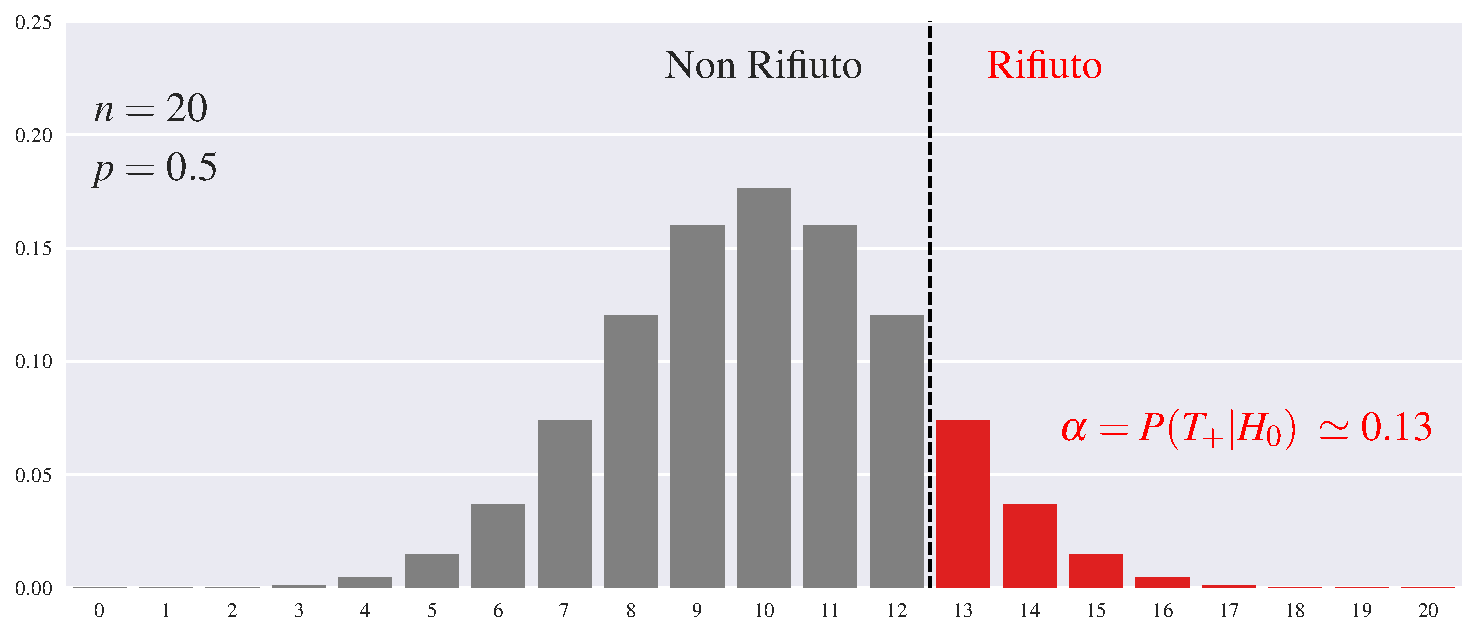
\includegraphics[width=0.9\textwidth]{figure/B-test_01.pdf}


%%%%%%%%%%%%
%%%%%%%%%%%%
%%%%%%%%%%%%
%%%%%%%%%%%%
\clearpage\hfill\textbf{Test Binomiale}\subsection{Testa una coda, errore II tipo}

La probabilità dei falsi negativi può essere espressa in funzione di $p$ (abbiamo solo assunto che $>1/2$)


\ceq{\hfill \Pr(T_-\mathrel|H_A)}{=}{\Pr(X< k\mathrel|H_A)\quad=\quad\sum^{k-1}_{i=1} {n\choose i}p^i(1-p)^{n-i}}

Se segliamo come prima $n=20$, $k=13$ abbiamo {\color{blue}\boldmath\ $T_-=\{0,\dots,12\}$} è la \emph{zona di NON rifiuto}.
Ora, per semplificare la discussione supponiamo di conoscere non solo il tipo ma anche la gravità del difetto. Quindi l'ipotesi alternativa diventa

$H_{3/4}:$\kern3ex $p=3/4$

Rappresentiamo la distribuzione di $X$ nel caso in cui vale $H_{3/4}$. Per confronto lo accostiamo al grafico del paragrafo precedente. 


\hfil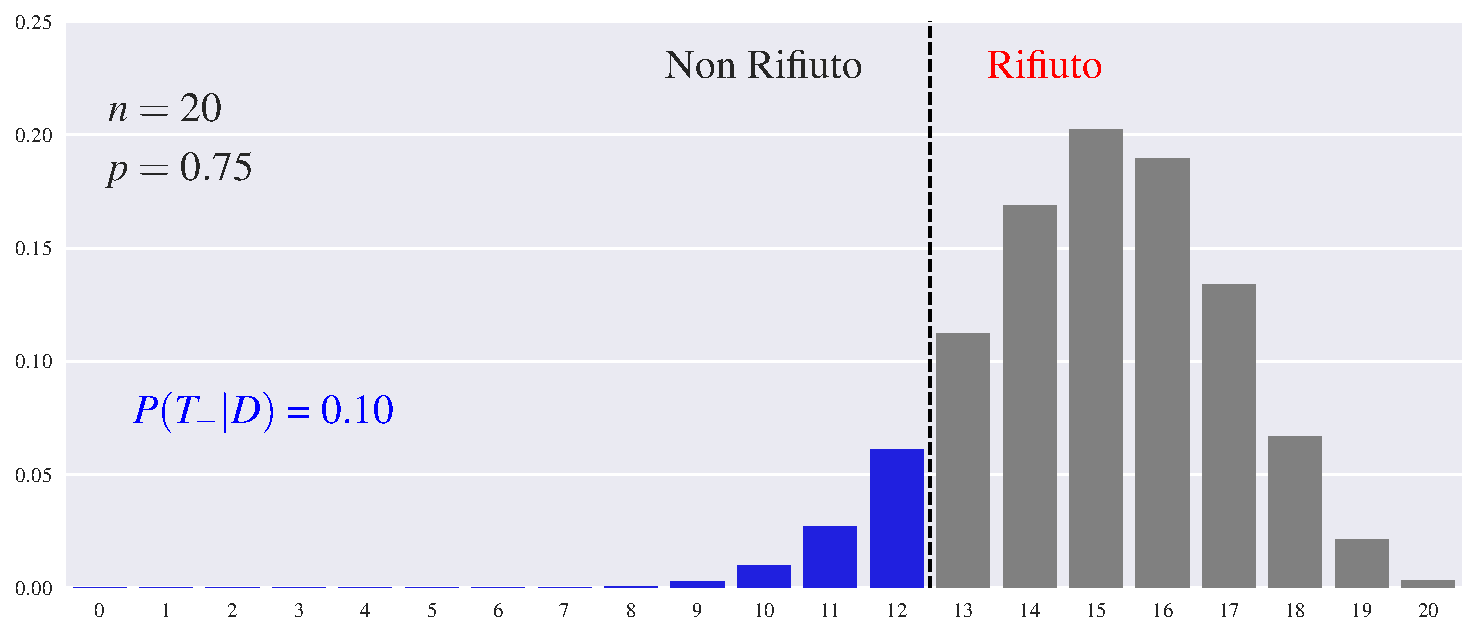
\includegraphics[width=0.9\textwidth]{figure/B-test_02.pdf}

\hfil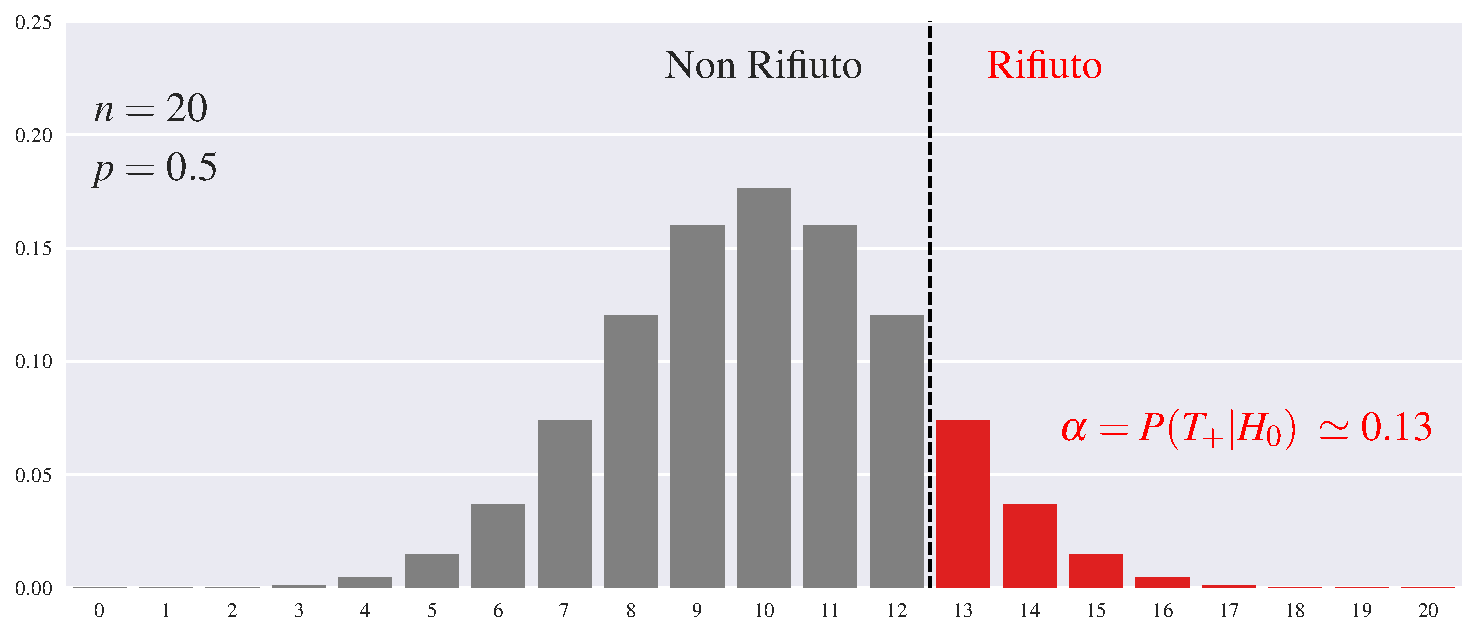
\includegraphics[width=0.9\textwidth]{figure/B-test_01.pdf}




%%%%%%%%%%%%
%%%%%%%%%%%%
%%%%%%%%%%%%
\clearpage\hfill\textbf{Test Binomiale}\subsection{Effect size: \boldmath{$\delta$}}


Cosa possiamo dire sul caso generale $H_A:$ $p>1/2$~?

Al crescere di $p$ la distribuzione si sposta verso destra quindi la probabilità di errori del II tipo diminuisce. Di converso, se $p$ si avvicina a $1/2$  la probabilità d'errore aumenta. Al limite quando $p\approx 1/2$ avremo $\alpha+\beta\approx 1$. Dobbiamo quindi fissare il minima differenza $\delta$ che riteniamo significativa e calcolare $\beta$ a paritire da quello.


\hfil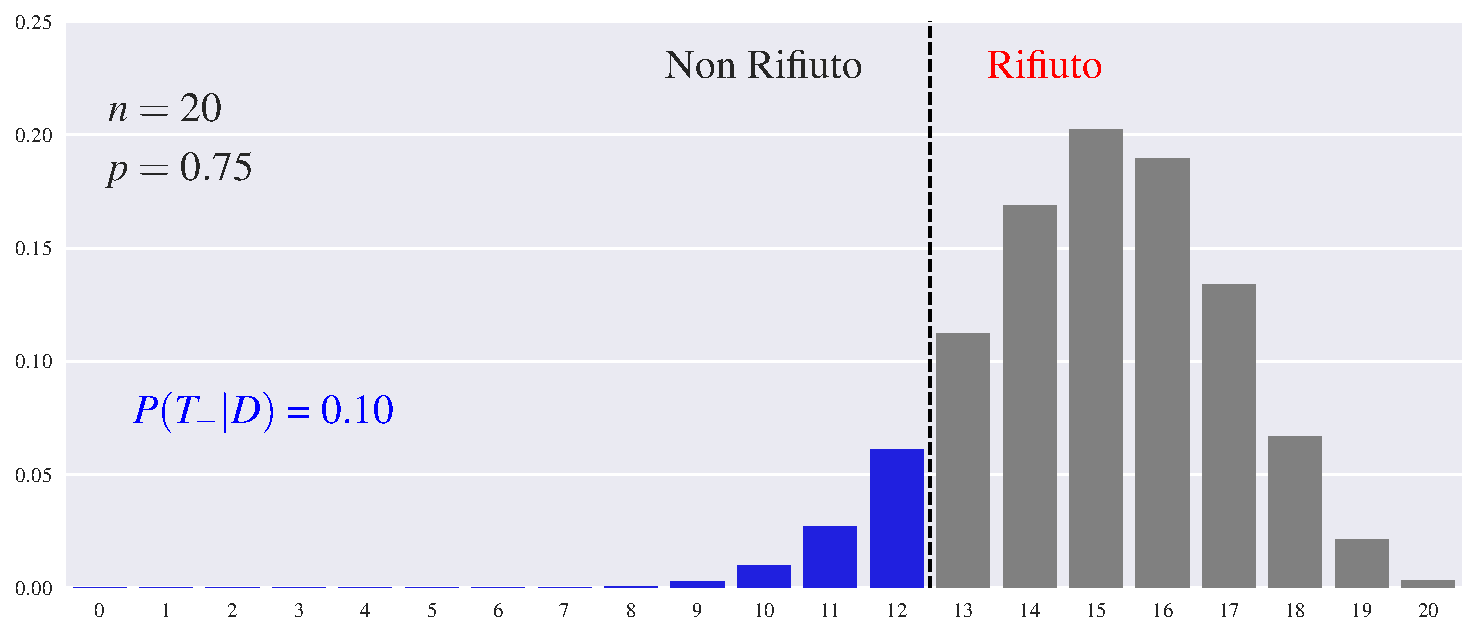
\includegraphics[width=0.9\textwidth]{figure/B-test_02.pdf}

\hfil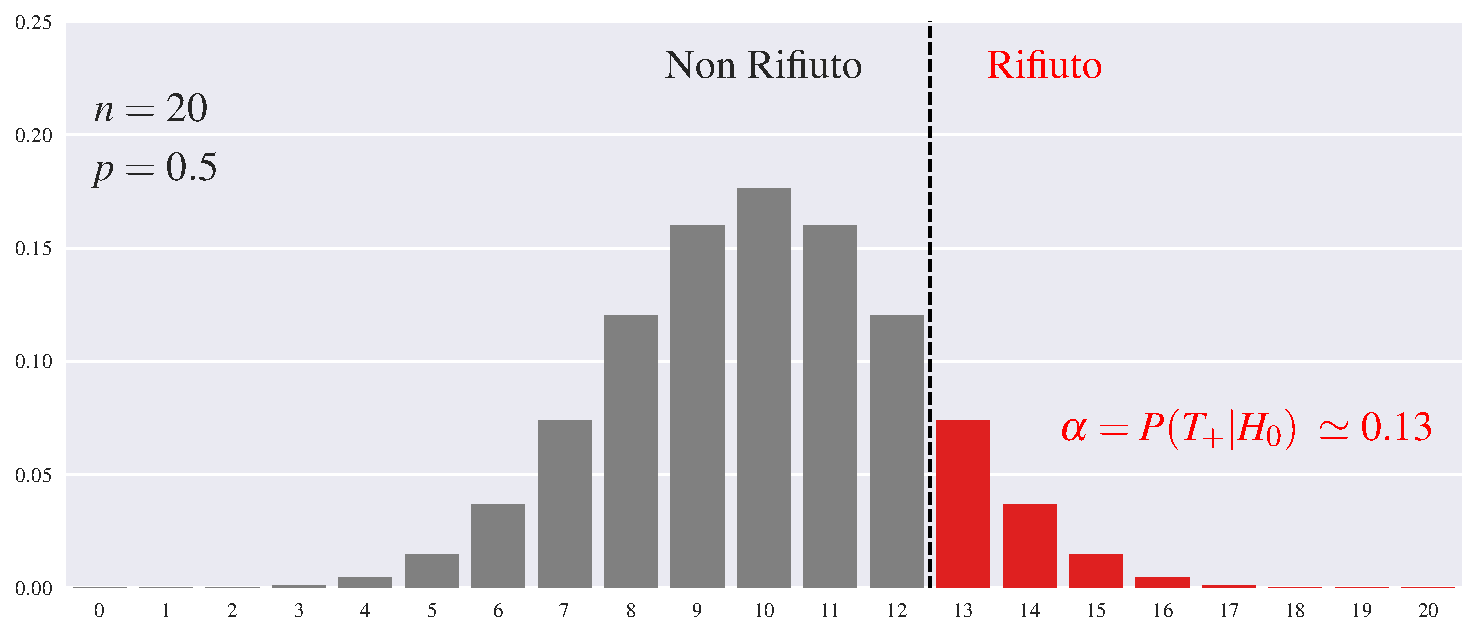
\includegraphics[width=0.9\textwidth]{figure/B-test_01.pdf}



%%%%%%%%%%%%
%%%%%%%%%%%%
%%%%%%%%%%%%
\clearpage\hfill\textbf{Test Binomiale}\subsection{Test a due code}

Nell'esempio precedente avevamo un'informazione certa sul tipo di difetto delle monete: sapevamo che $p>1/2$. Proviamo a fare senza, avremo quindi

$H_0:$\kern3.5ex $p=1/2$

$H_A:$\kern3ex $p\neq1/2$

Verifichiamo prima che  \textbf{la zona di rifiuto dei paragrafi precedenti NON è adatta\/} alla nuova situazione. L'analisi di $\Pr(T_+|H_0)$ rimane invariata (inaftti l'insieme $H_0$ non è cambiato).

Per semplificare la discussione dell'errore del II tipo supponiamo per il momento che 

$H_A:$\kern3ex $p=3/4$\quad o\quad $p=1/4$ 

Possiamo immaginare $H_A=H_{{1/4}}\cup H_{{3/4}}$. Se sostituiamo $H_A$ con $H_{{3/4}}$ il grafico rimane come quello già discusso. Ora però dobbiamo considerare il caso il cui la moneta appartenga all'insieme $H_{{1/4}}$

\hfil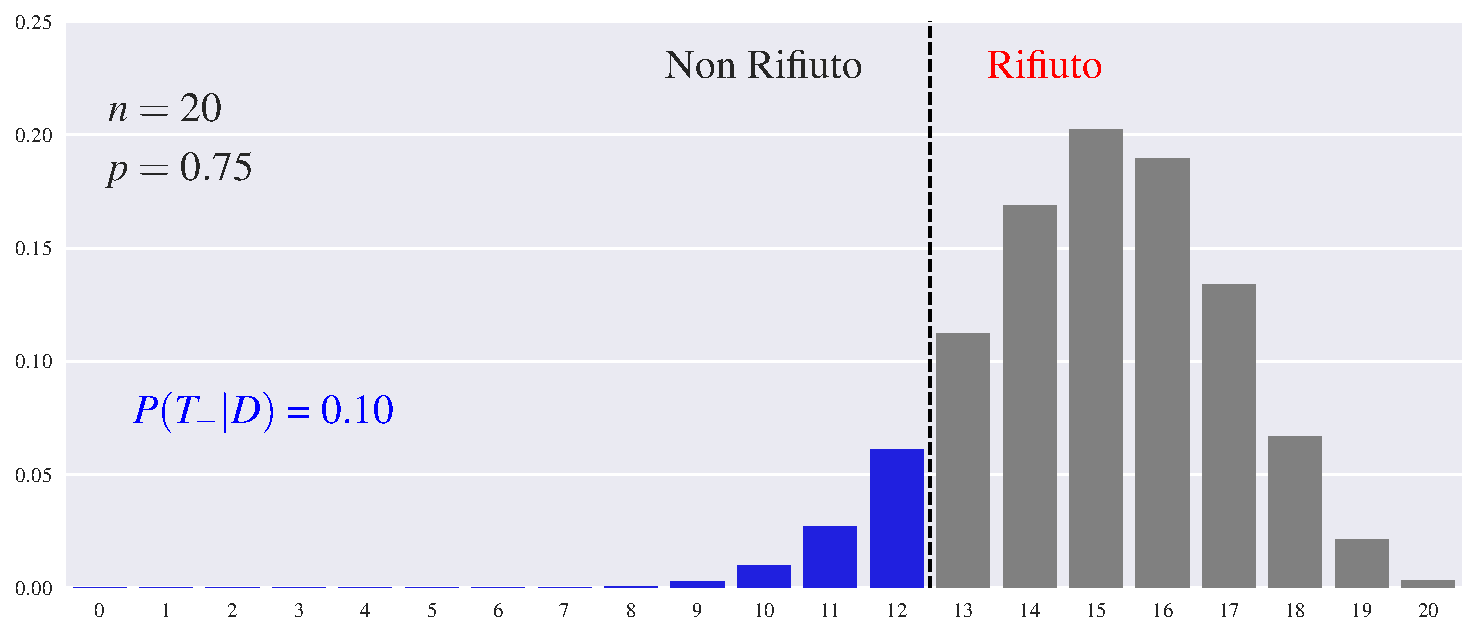
\includegraphics[width=0.9\textwidth]{figure/B-test_02.pdf}

\hfil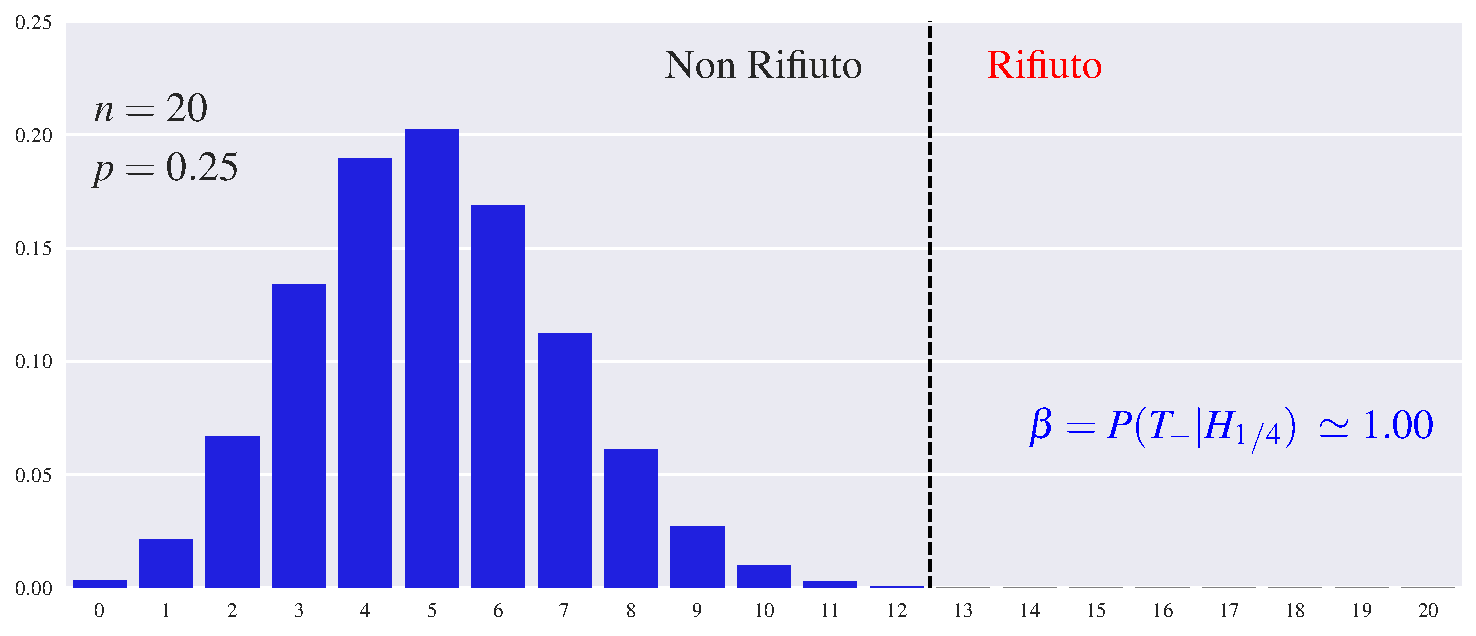
\includegraphics[width=0.9\textwidth]{figure/B-test_03.pdf}


%%%%%%%%%%%%
%%%%%%%%%%%%
%%%%%%%%%%%%
\clearpage\hfill\textbf{Test Binomiale}\subsection{Test a due code, errori I e II tipo}

Per riparare il problema discusso al paragrafo precedente. prendiamo come zona di rifiuto $T_+=\{0,\dots,7=n-k\}\cup \{k=13,\dots,20=n\}$

\hfil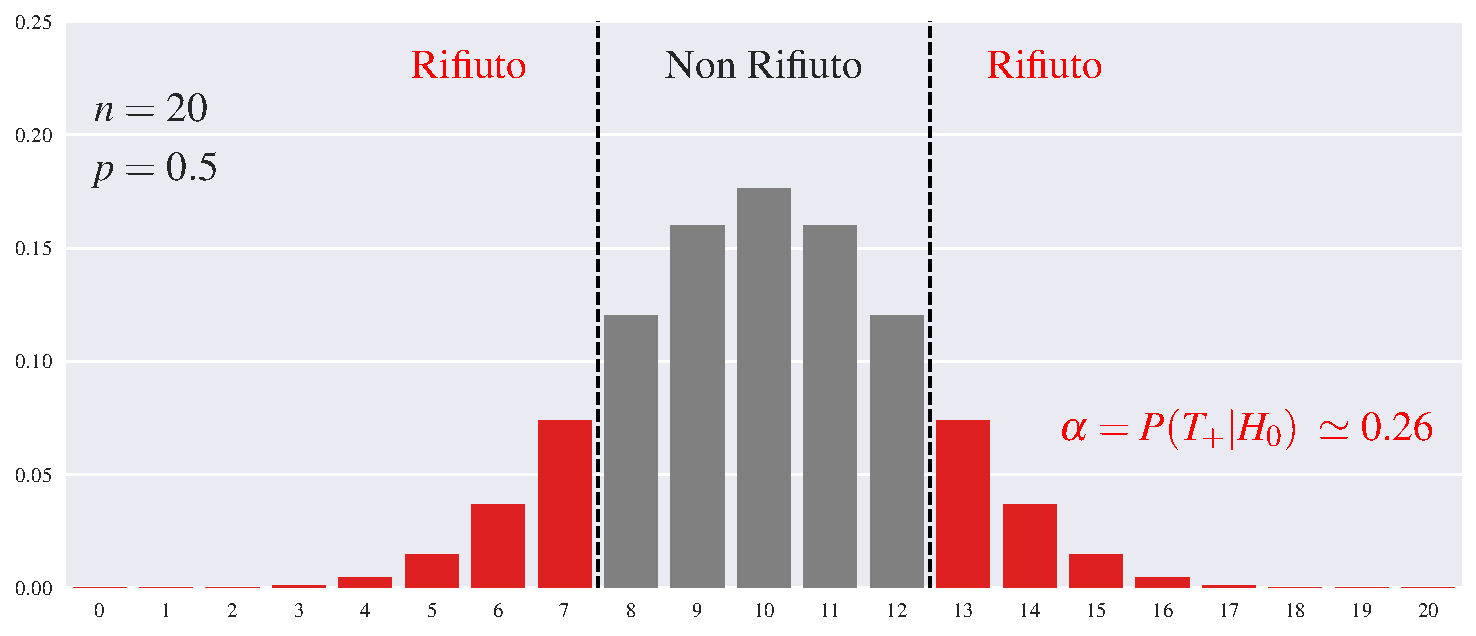
\includegraphics[width=0.9\textwidth]{figure/B-test_04.pdf}

\hfil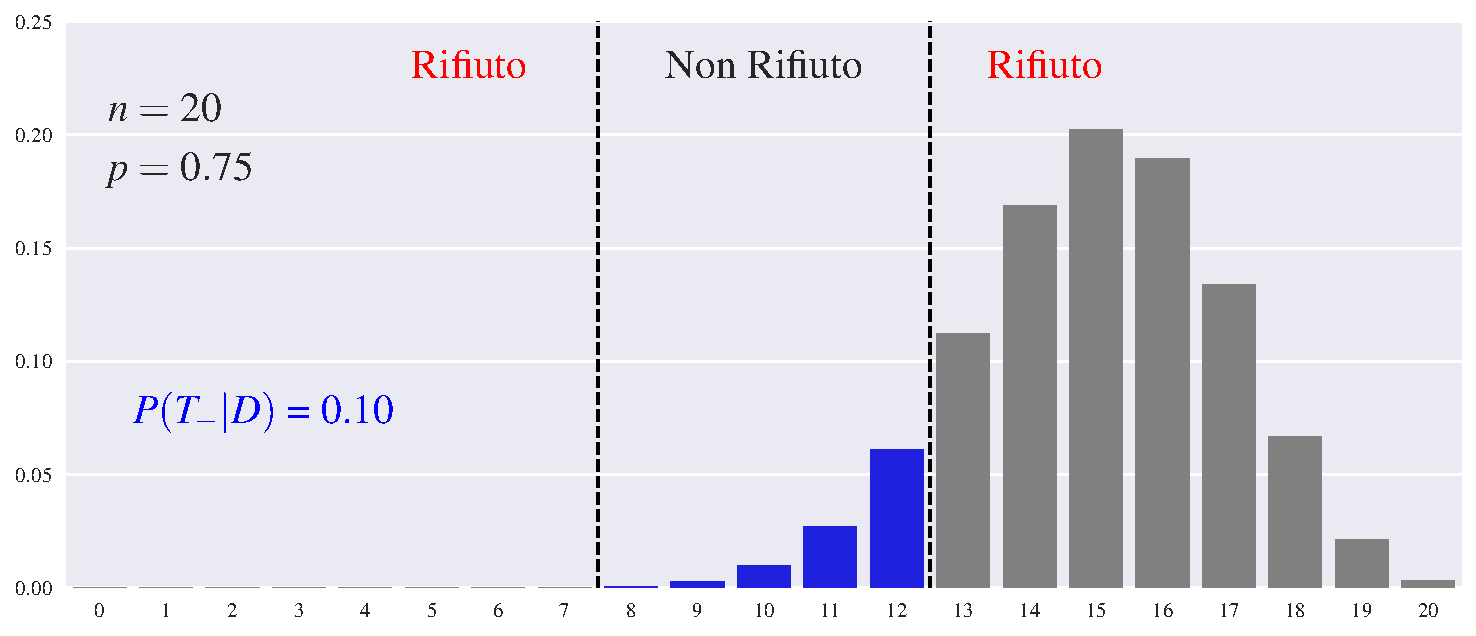
\includegraphics[width=0.9\textwidth]{figure/B-test_05.pdf}

\hfil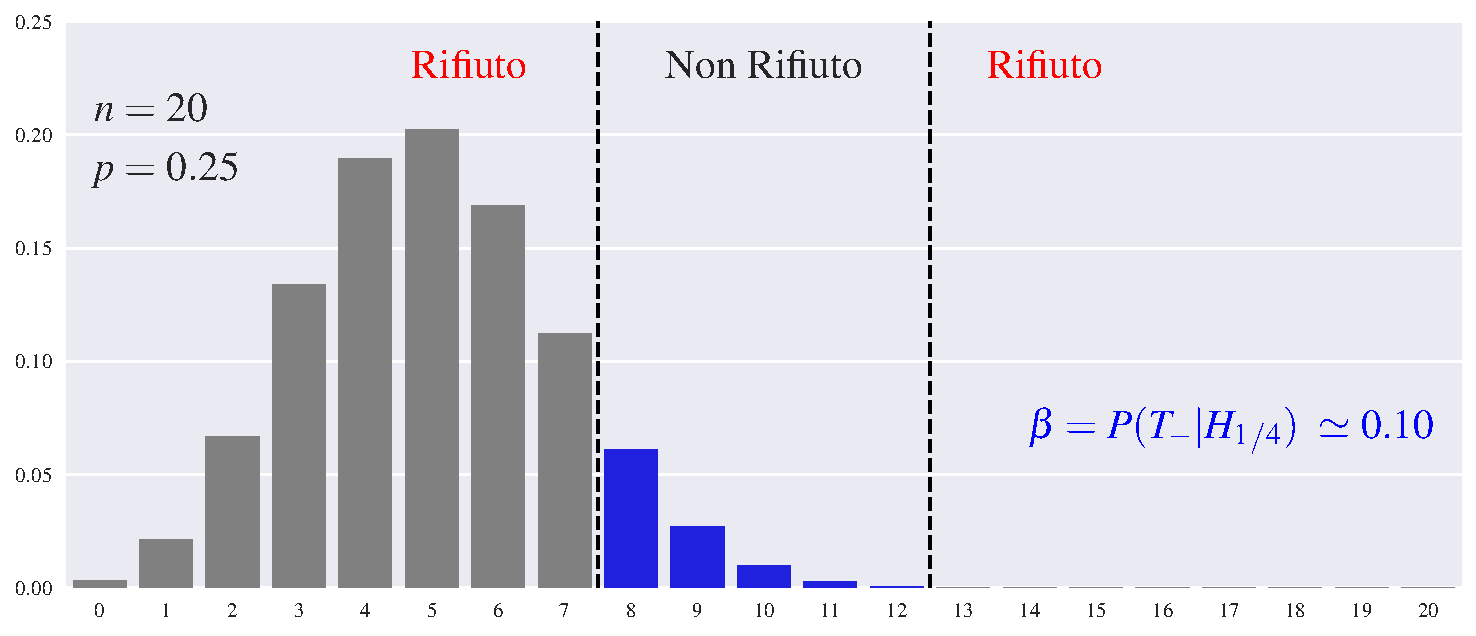
\includegraphics[width=0.9\textwidth]{figure/B-test_06.pdf}




%%%%%%%%%%%%
%%%%%%%%%%%%
%%%%%%%%%%%%
\clearpage\hfill\textbf{Test Binomiale}
\subsection{Test a due code, con campione più ampio}

Supponiamo di raddoppiare la dimensione del campione ($n=40$). Aggiustiamo la zona di rifiuto allo stesso modo ($k=26$):  $T_+=\{0,\dots,14=n-k\}\cup \{k=26,\dots,40=n\}$

Entrambi gli errori diminuiscono.


\hfil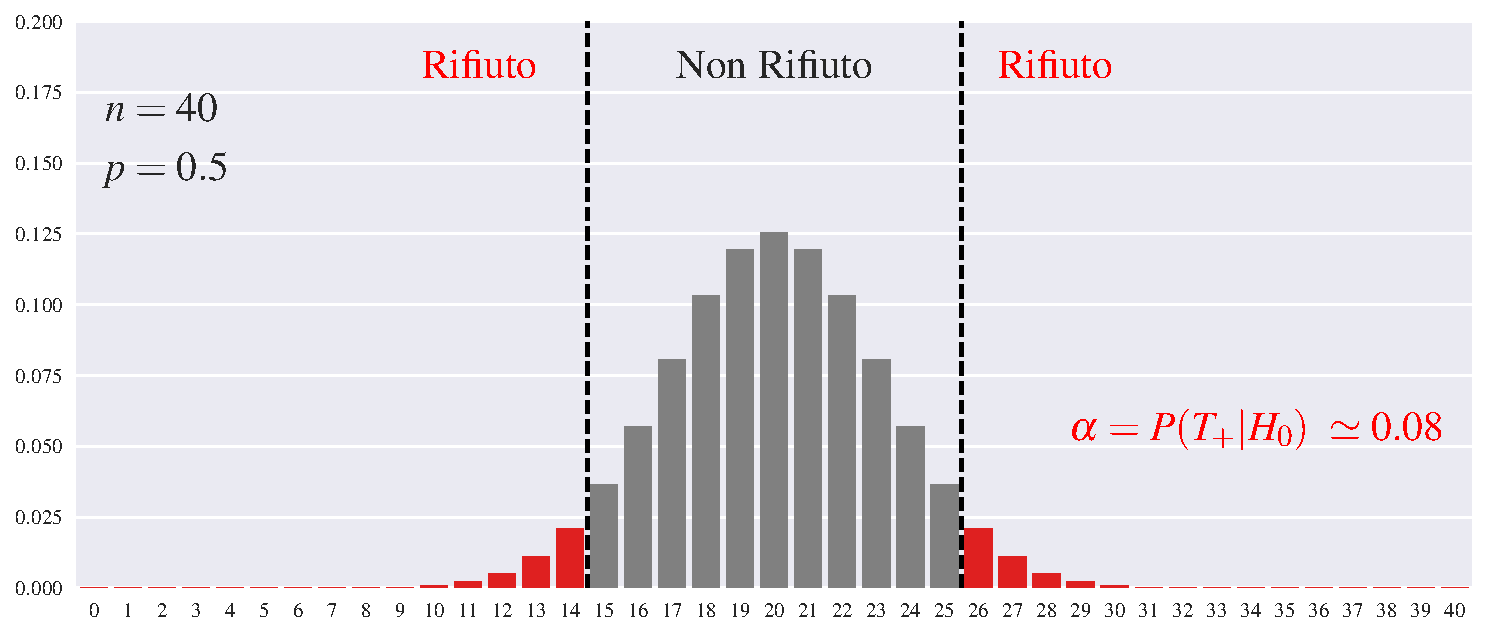
\includegraphics[width=0.9\textwidth]{figure/B-test_07.pdf}

\hfil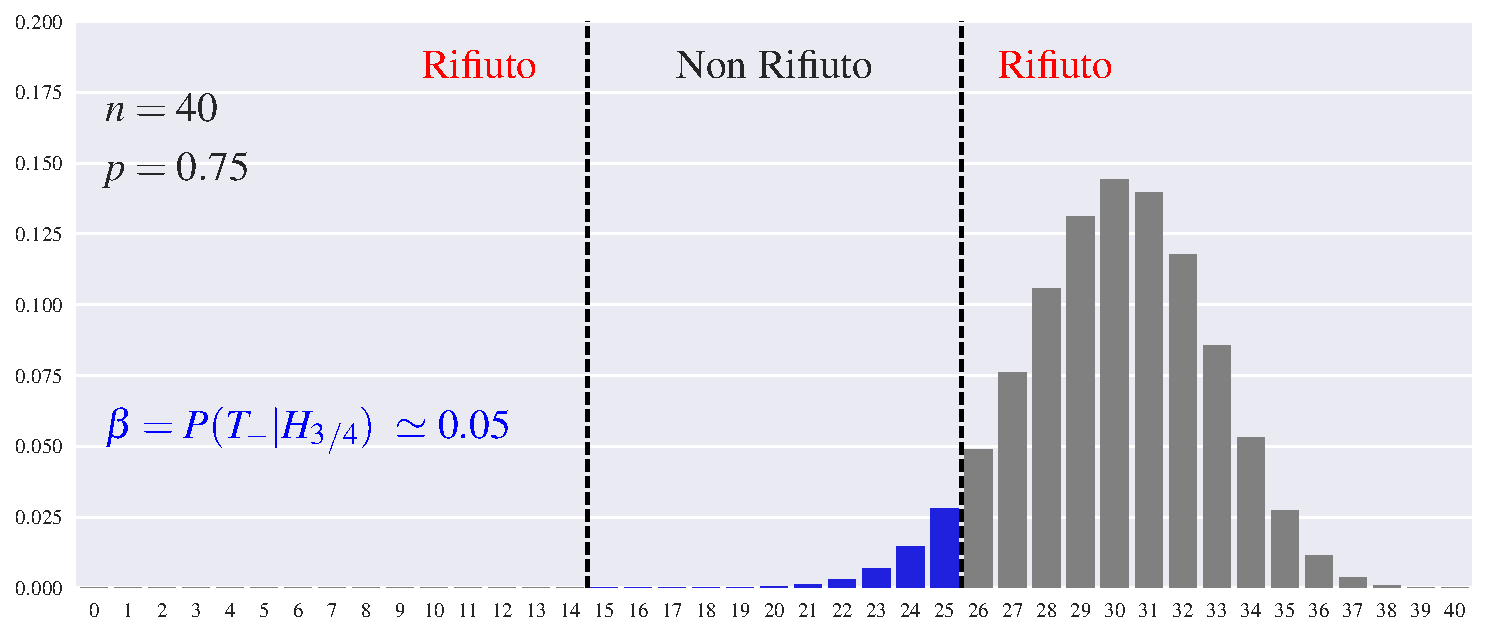
\includegraphics[width=0.9\textwidth]{figure/B-test_08.pdf}

\hfil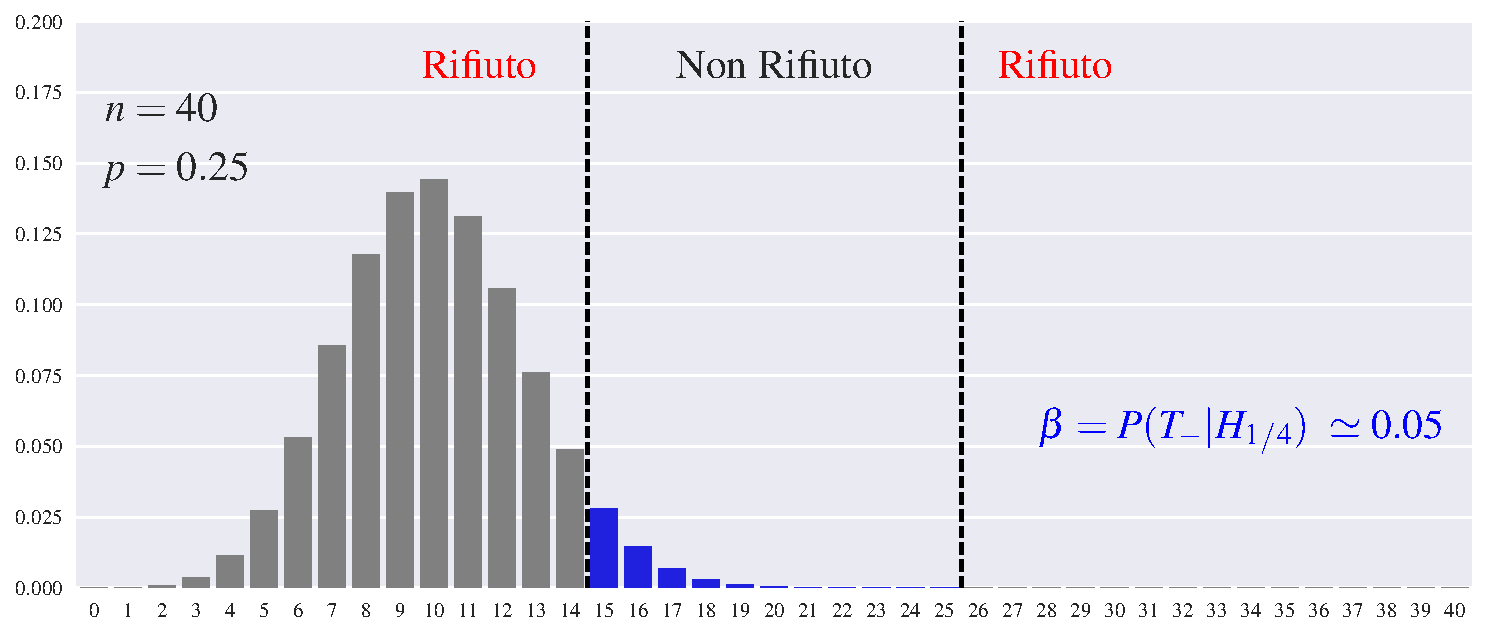
\includegraphics[width=0.9\textwidth]{figure/B-test_09.pdf}




%%%%%%%%%%%%
%%%%%%%%%%%%
%%%%%%%%%%%%
\clearpage\hfill\textbf{Test Binomiale}
\subsection{Standardizzazione (1)}

Il confronto tra i test con $n=20, 40$ non é immediato (vedi la trasformazione della zona di rifiuto). Per facilitare il confronto tipicamente la variabile viene standardizzata. 

Se $X\sim B(n,p)$ allora, ricordando che la media è $\mu=np$ e la varianza è $\sigma^2=np(1-p)$, la variabile standardizzata diventa

\ceq{\hfill Z}{=}{\frac{X-\mu}{\sigma}}

\ceq{\hfill }{=}{\frac{X-np}{\rule{0ex}{3ex}\sqrt{np\big(1-p\big)}}}


Gli esempi considerati (con $n=20,40$ e $k=13,26$) diventano: 

\hfil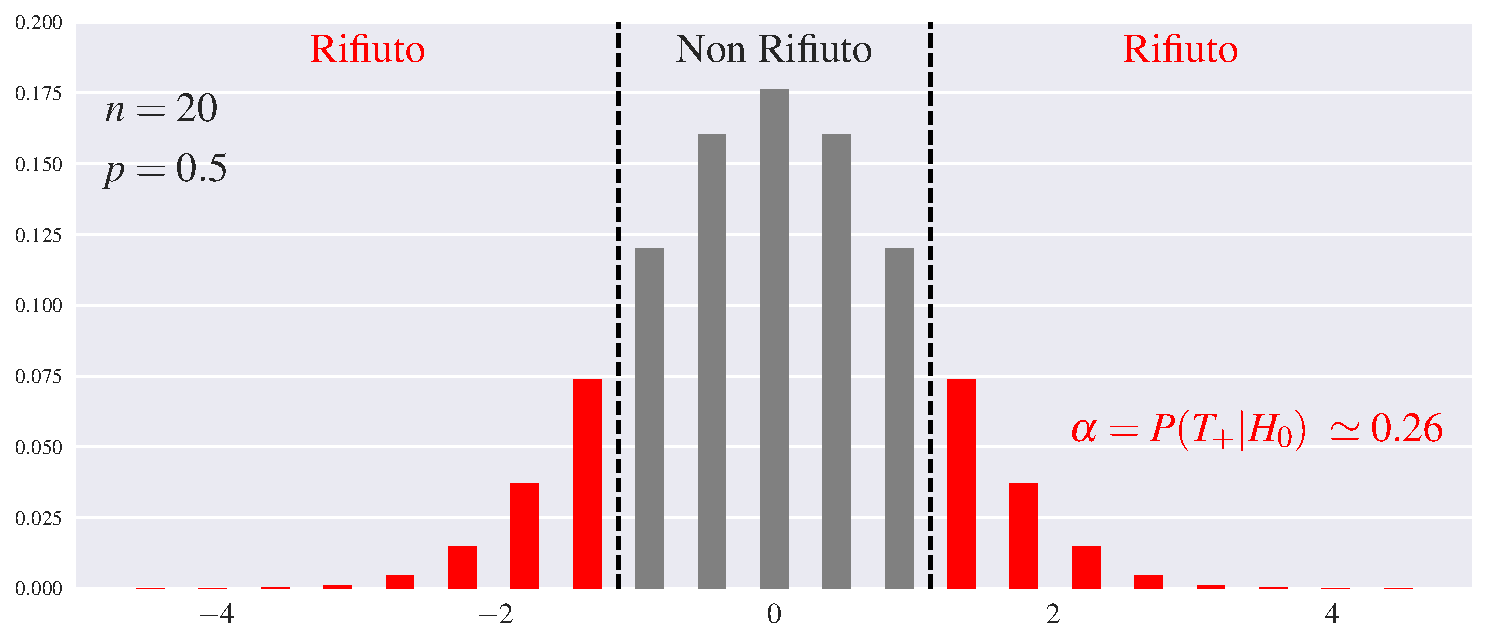
\includegraphics[width=0.9\textwidth]{figure/B-test-standard_01.pdf}

\hfil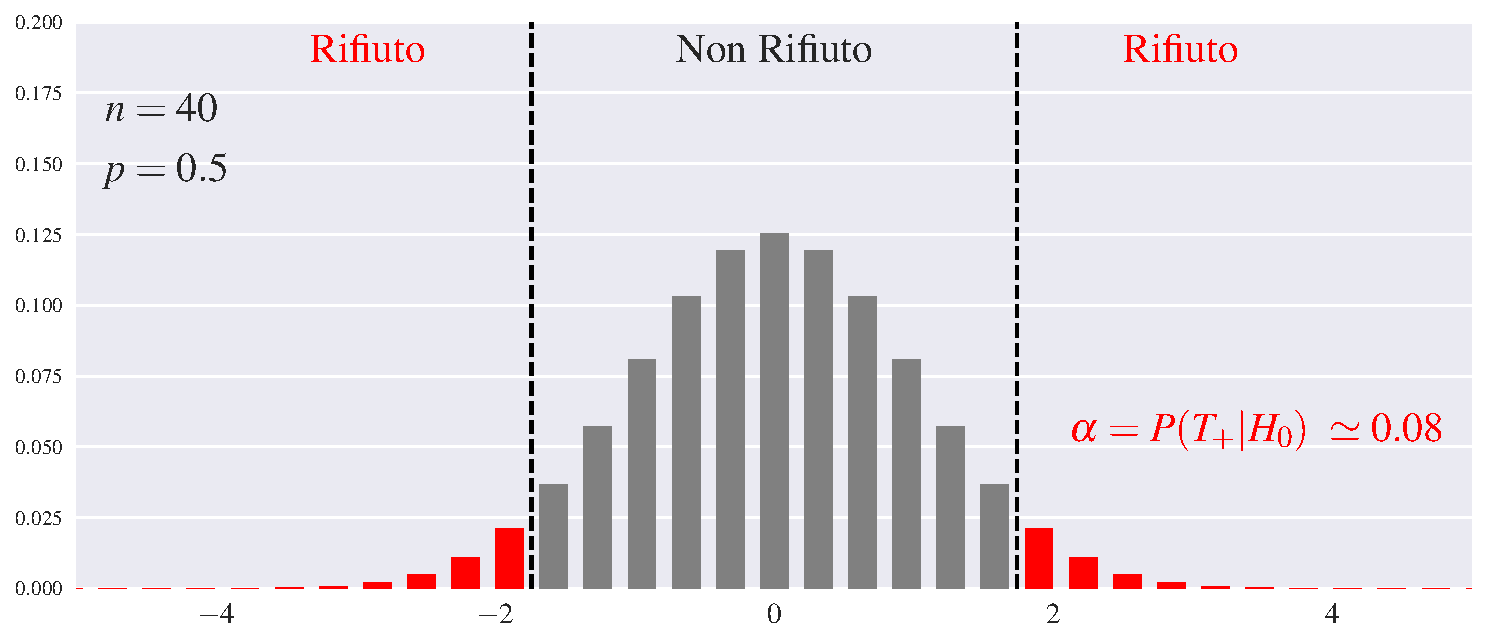
\includegraphics[width=0.9\textwidth]{figure/B-test-standard_02.pdf}


%%%%%%%%%%%%
%%%%%%%%%%%%
%%%%%%%%%%%%
\clearpage\hfill\textbf{Test Binomiale}
\subsection{Standardizzazione (2)}

Si noti che le regioni di rifiuto non sono le stesse. in effetti


\ceq{\hfill\frac{k-np}{\rule{0ex}{3ex}\sqrt{np\big(1-p\big)}}}{=}{1.34}\qquad se $n=20$, \ $k=13$, \ $p=05$


\ceq{}{=}{1.90}\qquad se $n=40$, \ $k=26$, \ $p=05$


Se per entriambi i casi prendiamo la stessa regione di rifiuto misurata in punteggio $Z$, diciamo $(-\infty, -1.34]\ \cup\ [1.34, +\infty)]$ avremmo ottenuto praticamente lo stesso $\alpha$. Infatti una volta standardizzate le due distribuzioni diventano estremamente simili. Lo scopo dela standardizzazione è rendere evidenti queste similitudini.  


\hfil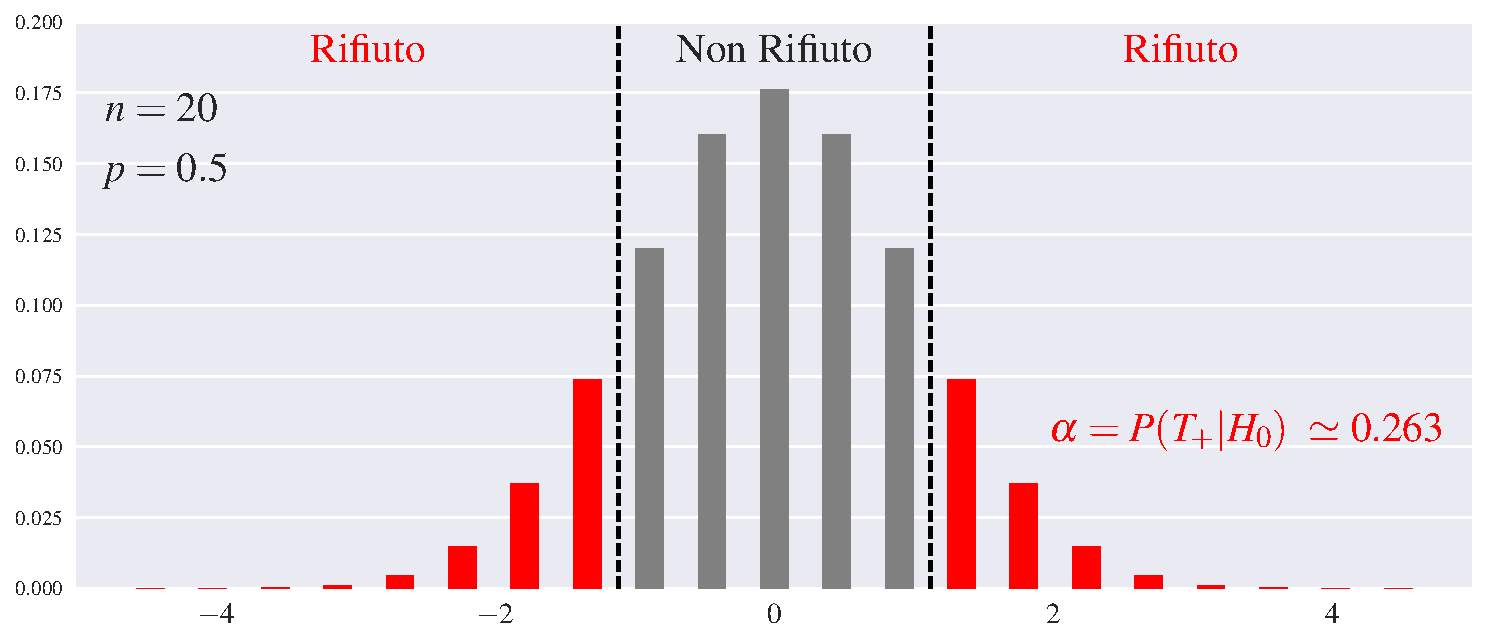
\includegraphics[width=0.9\textwidth]{figure/B-test-standard2_01.pdf}

\hfil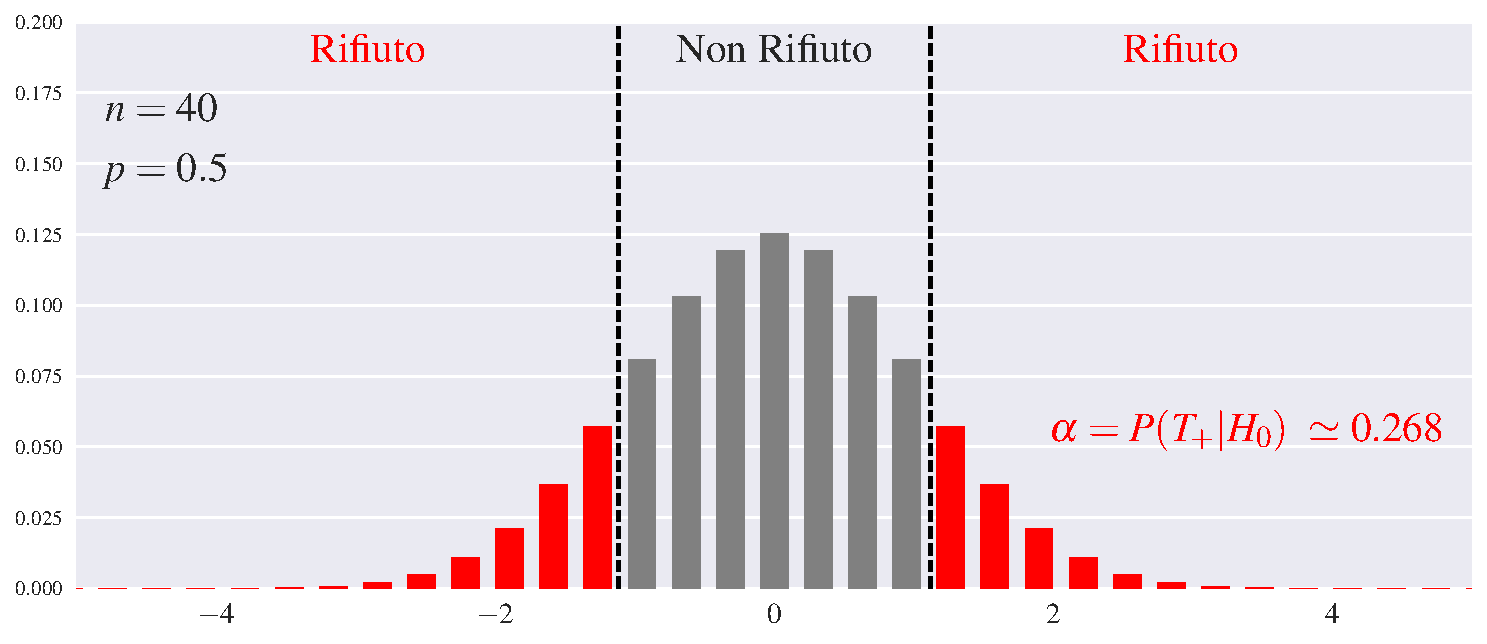
\includegraphics[width=0.9\textwidth]{figure/B-test-standard2_02.pdf}




%%%%%%%%%%%%
%%%%%%%%%%%%
%%%%%%%%%%%%
\clearpage
\section{Z-test}
\subsection{Una coda}

Si sospetta che una certa terapia faccia aumentare la pressione diastolica. Nella popolazione generale la pressione diastolica ha distribuzione $N(\mu_0,\sigma^2)$ con $\mu_0=75$ e $\sigma=9.5$. 

Assumiamo che tra i pazienti in terapia la pressione diastolica sia distribuita normalmente con media ignota $\mu$ e con la stessa deviazione standard della popolazione generale. Vogliamo testare le seguenti ipotesi:

$H_0:$\kern3.5ex $\mu=\mu_0$

$H_A:$\kern3ex $\mu>\mu_0$

Il test consiste nel misurare la pressione ad un campione di $n$ pazienti e di questi dati calcolare la media. Abbiamo quindi la seguente statistica

\ceq{\hfill \bar X}{=}{\frac1n\sum_{i=1}^nX_i}

Dove $X_i$ è la v.a.\@ che dà la pressione dell'$i$-esimo pazione del campione. Rigetteremo $H_0$ se il valore ottenuto è suporiore ad un certo $x_\alpha$ che vogliamo fissare in modo che l'errore I tipo risulti uguale ad $\alpha$. Quindi $x_\alpha$ dev'essere tale che $x_\alpha$ tale che $\Pr(\bar X>x_\alpha)=\alpha$.

Se $H_0$ è vera, $\bar X\sim N\bigg(\mu_0,\dfrac{\sigma^2}{n}\bigg)$.

% Non è necessario, ma conviene sempre ridursi alla normale standard: $\dfrac{\bar X-\mu_0}{\sigma/\sqrt{n}}$ ha distribuzione normale standard $Z$.
% 
% Vogliamo $x_\alpha$ tale che $\Pr(Z>\dfrac{x_\alpha-\mu_0}{\sigma/\sqrt{n}})=\alpha$



%%%%%%%%%%%%
%%%%%%%%%%%%
%%%%%%%%%%%%
\clearpage\subsection{Una coda, errore I e II tipo\hfill Z-test}


Qui rappresentiamo gli errori del I e II tipo per campioni di dimensione $n=20, 40$. Per gli errori del II tipo prendiamo $\delta=5$.

\hfil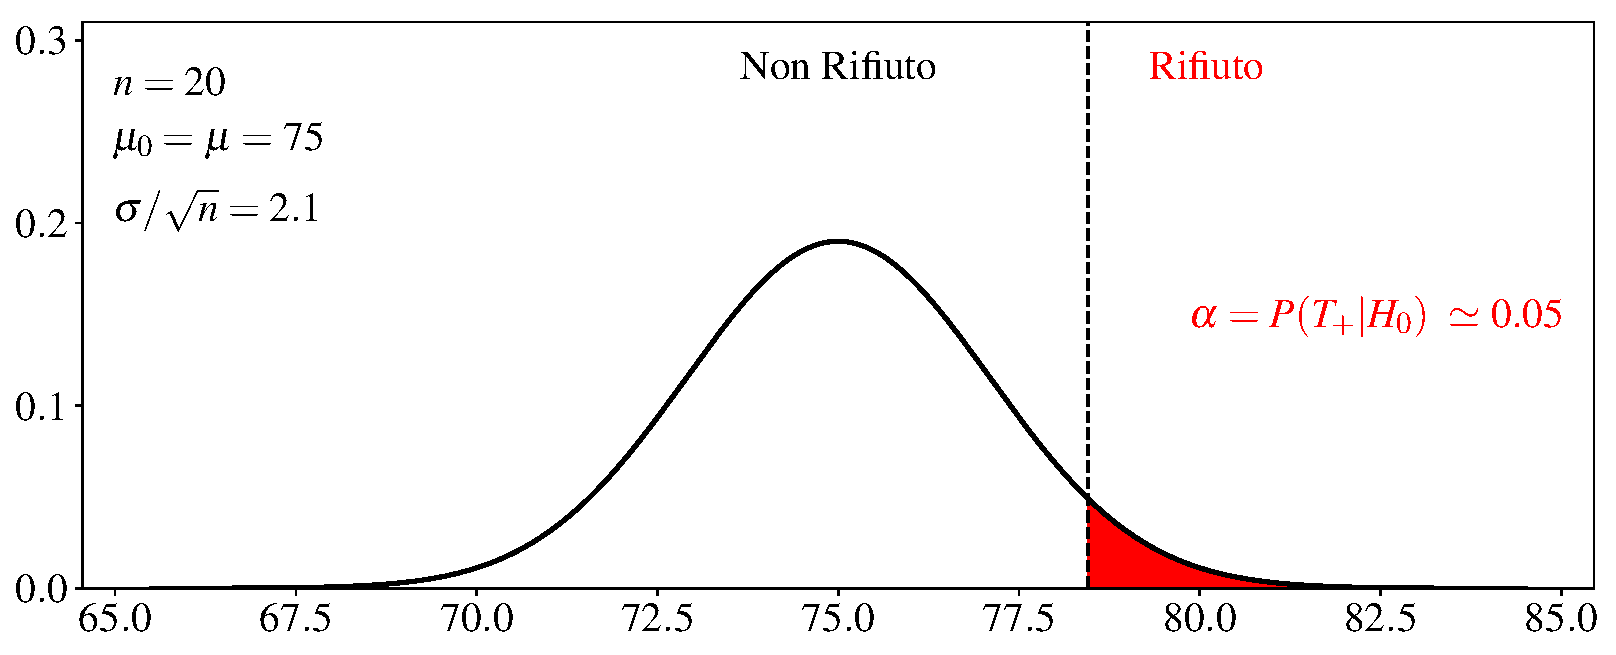
\includegraphics[width=0.8\textwidth]{figure/Z-test_01.pdf}

\hfil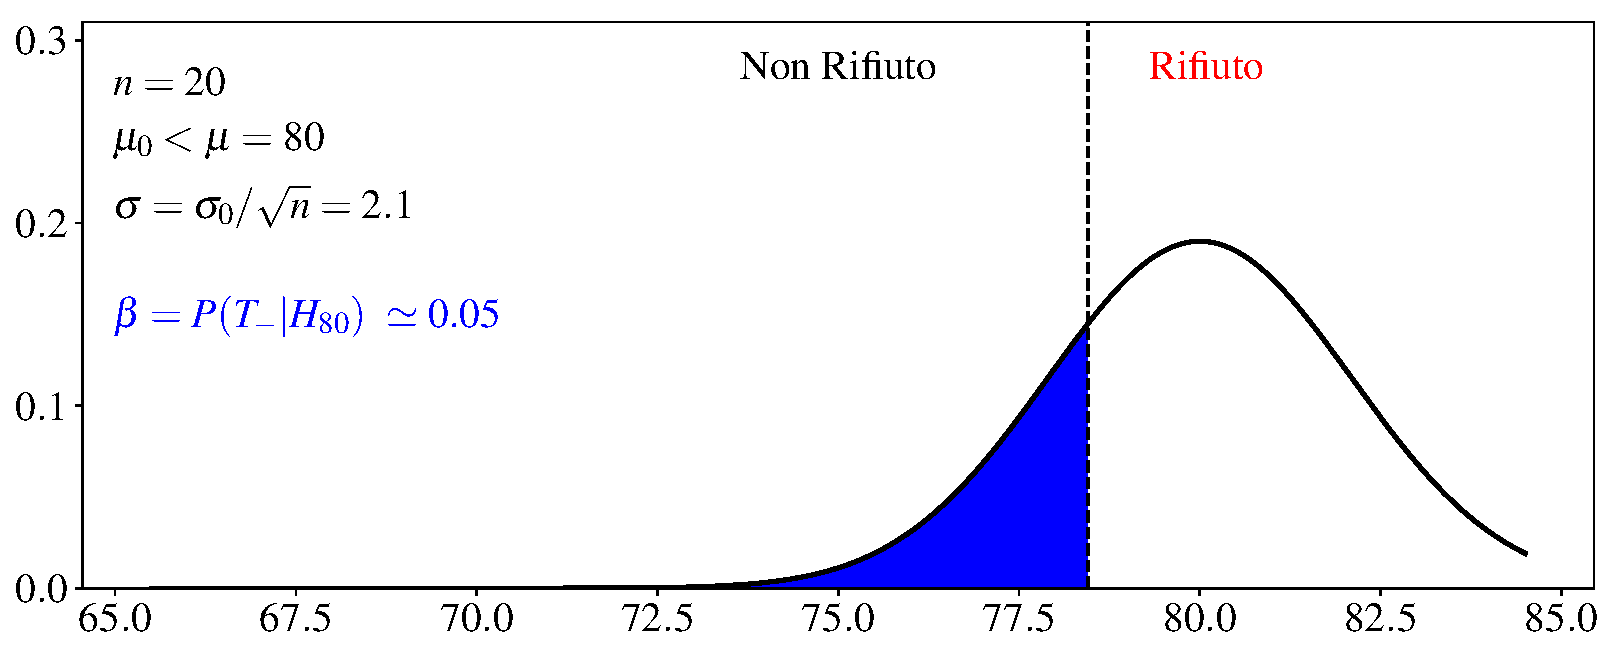
\includegraphics[width=0.8\textwidth]{figure/Z-test_02.pdf}

\hfil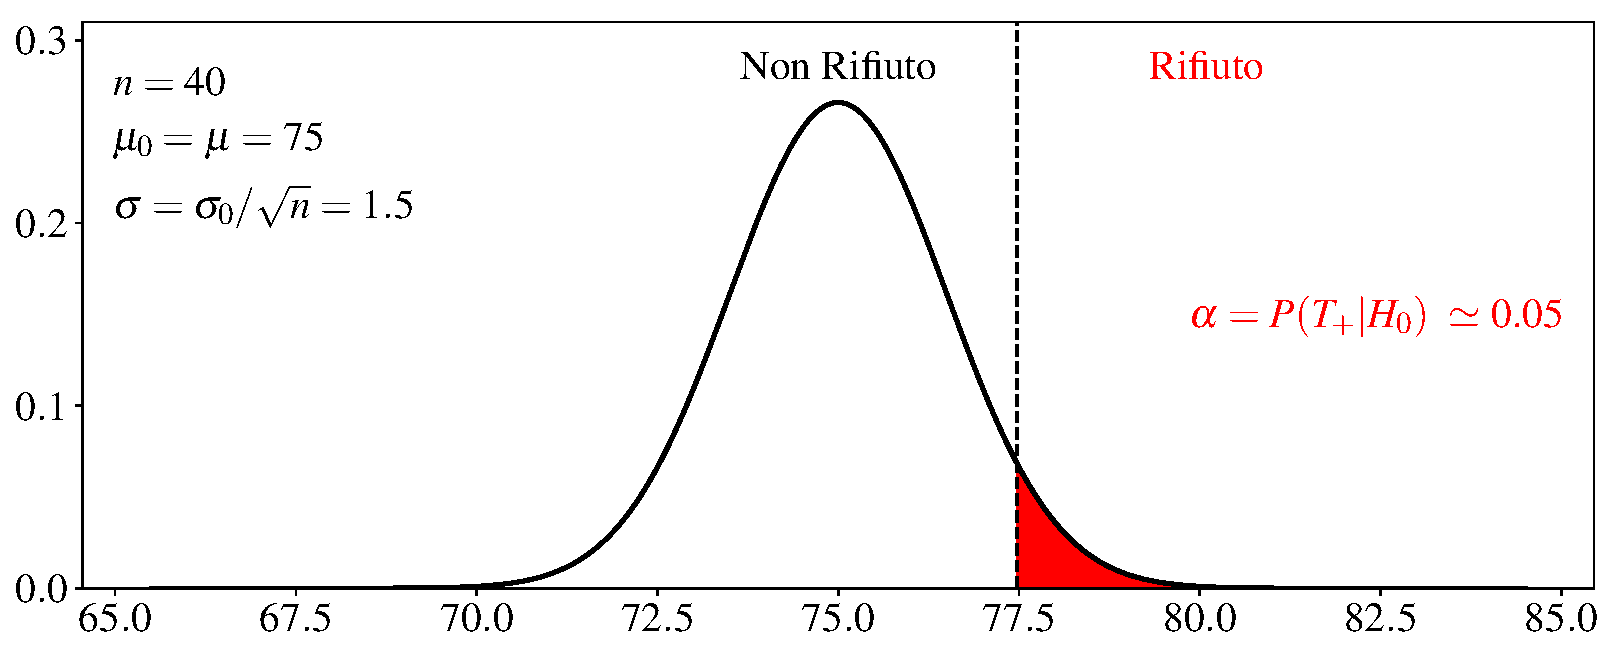
\includegraphics[width=0.8\textwidth]{figure/Z-test_03.pdf}

\hfil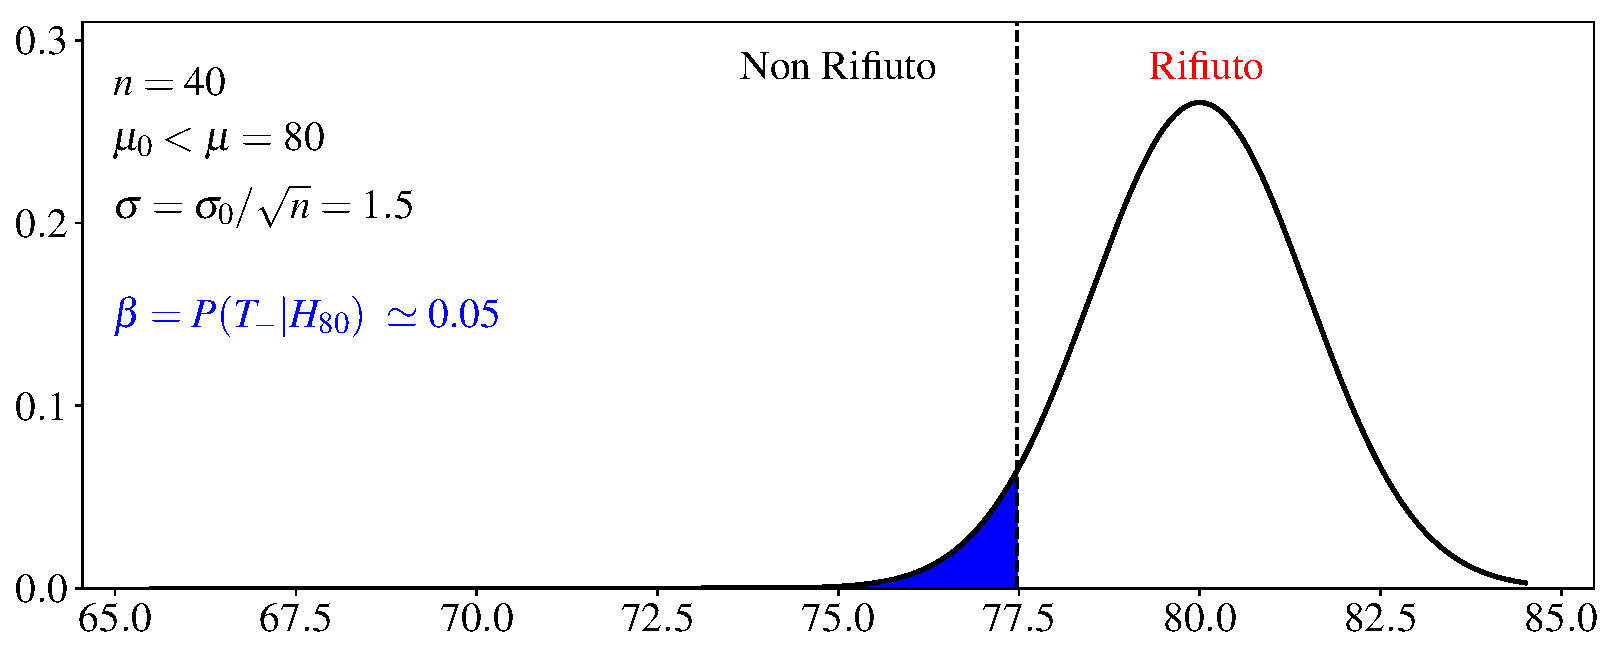
\includegraphics[width=0.8\textwidth]{figure/Z-test_04.pdf}





%%%%%%%%%%%%
%%%%%%%%%%%%
%%%%%%%%%%%%
\clearpage\subsection{Una coda, p valore.\hfill Z-test}


Supponiamo di ottenere $\bar x=78.0$ da un campione di dimensione $n=40$. Il p-valore di questa misura è $\Pr(\bar X>78)=1-\Pr(\bar X\le 78)$.





%%%%%%%%%%%%
%%%%%%%%%%%%
%%%%%%%%%%%%
\clearpage\section{Esercizi vari}
\subsection{Placebo\hfill Esercizi}


Ad un gruppo di persone vengono misurati 50 diversi parametri fisiologici (che assumiamo indipendenti) prima e dopo l'assunzione di un placebo. Per ognuno di questi parametri l'ipotesi nulla è che non ci sia differenza. Qual'è la probabilità che per almeno uno di questi parametri si ottenga p-valore $<0.02$~?


Risposta:\kern3ex $1-(0.98)^{50}=64\%$


\section{Inferenza Bayesiana}

In un casinó si gioca a testa o croce ($1$ o $0$) con tre tipi di monete che hanno probabilità di successo $1/2$, $2/3$, e $1/3$. Il casinò sceglie la moneta e continua a giocare con la stessa moneta per tutto il giorno. Il giocatore non sa quale moneta sia scelta.

Assumiamo per fissare le idee che il casinò scelga la monete a sorte e che le tre monete abbiano la stessa probabilità di essere scelte. Supponiamo osservare la sequenza $010$ e di voler puntare sul prossimo lancio. Ci interessa sapere con che probabilità possiamo assumere quale moneta.  

Siano $M_{1/2}$, $M_{2/3}$ ed $M_{1/3}$ gli eventi che corrispondono alla scelta delle tre monete
$M_{1/2}$, $M_{2/3}$ ed $M_{1/3}$

$\Pr(010\mathrel|M_{1/2})\ =\ \dfrac{1}{2^3}\ =\ \dfrac{1}{8}$

$\Pr(010\mathrel|M_{2/3})\ =\ \dfrac{1}{3}\cdot\dfrac{2}{3}\cdot\dfrac{1}{3}\ =\ \dfrac{2}{9}$

$\Pr(010\mathrel|M_{1/3})\ =\ \dfrac{2}{3}\cdot\dfrac{1}{3}\cdot\dfrac{2}{3}\ =\ \dfrac{4}{9}$

\smallskip
Usando il teorema delle probabilità totali possiamo facilmente calcolare 

$\Pr(010)\ =\ \dfrac{1}{3}\left(\dfrac{1}{8}+\dfrac{2}{9}+\dfrac{4}{9}\right)\ =\ \dfrac{19}{72}$.

Quindi possiamo calcolare la probabilità di $M_{1/2}$, $M_{2/3}$ ed $M_{1/3}$ data l'informazione $010$.

$\Pr(M_{1/2} \mathrel| 010)=\dfrac{\Pr(010\mathrel|M_{1/2})\cdot \Pr(M_{1/2})}{\Pr(010)}=\dfrac{1/8\cdot 1/3}{19/72}$

$\Pr(M_{2/3} \mathrel| 010)=\dfrac{\Pr(010\mathrel|M_{2/3})\cdot \Pr(M_{2/3})}{\Pr(010)}=\dfrac{2/9\cdot 1/3}{19/72}$

$\Pr(M_{1/3} \mathrel| 010)=\dfrac{\Pr(010\mathrel|M_{1/3})\cdot \Pr(M_{1/3})}{\Pr(010)}=\dfrac{4/9\cdot 1/3}{19/72}$




\end{document}
